
%% bare_conf.tex
%% V1.3
%% 2007/01/11
%% by Michael Shell
%% See:
%% http://www.michaelshell.org/
%% for current contact information.
%%
%% This is a skeleton file demonstrating the use of IEEEtran.cls
%% (requires IEEEtran.cls version 1.7 or later) with an IEEE conference paper.
%%
%% Support sites:
%% http://www.michaelshell.org/tex/ieeetran/
%% http://www.ctan.org/tex-archive/macros/latex/contrib/IEEEtran/
%% and
%% http://www.ieee.org/

%%*************************************************************************
%% Legal Notice:
%% This code is offered as-is without any warranty either expressed or
%% implied; without even the implied warranty of MERCHANTABILITY or
%% FITNESS FOR A PARTICULAR PURPOSE! 
%% User assumes all risk.
%% In no event shall IEEE or any contributor to this code be liable for
%% any damages or losses, including, but not limited to, incidental,
%% consequential, or any other damages, resulting from the use or misuse
%% of any information contained here.
%%
%% All comments are the opinions of their respective authors and are not
%% necessarily endorsed by the IEEE.
%%
%% This work is distributed under the LaTeX Project Public License (LPPL)
%% ( http://www.latex-project.org/ ) version 1.3, and may be freely used,
%% distributed and modified. A copy of the LPPL, version 1.3, is included
%% in the base LaTeX documentation of all distributions of LaTeX released
%% 2003/12/01 or later.
%% Retain all contribution notices and credits.
%% ** Modified files should be clearly indicated as such, including  **
%% ** renaming them and changing author support contact information. **
%%
%% File list of work: IEEEtran.cls, IEEEtran_HOWTO.pdf, bare_adv.tex,
%%                    bare_conf.tex, bare_jrnl.tex, bare_jrnl_compsoc.tex
%%*************************************************************************

% *** Authors should verify (and, if needed, correct) their LaTeX system  ***
% *** with the testflow diagnostic prior to trusting their LaTeX platform ***
% *** with production work. IEEE's font choices can trigger bugs that do  ***
% *** not appear when using other class files.                            ***
% The testflow support page is at:
% http://www.michaelshell.org/tex/testflow/



% Note that the a4paper option is mainly intended so that authors in
% countries using A4 can easily print to A4 and see how their papers will
% look in print - the typesetting of the document will not typically be
% affected with changes in paper size (but the bottom and side margins will).
% Use the testflow package mentioned above to verify correct handling of
% both paper sizes by the user's LaTeX system.
%
% Also note that the "draftcls" or "draftclsnofoot", not "draft", option
% should be used if it is desired that the figures are to be displayed in
% draft mode.
%
\documentclass[conference]{IEEEtran}
% Add the compsoc option for Computer Society conferences.
%
% If IEEEtran.cls has not been installed into the LaTeX system files,
% manually specify the path to it like:
% \documentclass[conference]{../sty/IEEEtran}





% Some very useful LaTeX packages include:
% (uncomment the ones you want to load)


% *** MISC UTILITY PACKAGES ***
%
%\usepackage{ifpdf}
% Heiko Oberdiek's ifpdf.sty is very useful if you need conditional
% compilation based on whether the output is pdf or dvi.
% usage:
% \ifpdf
%   % pdf code
% \else
%   % dvi code
% \fi
% The latest version of ifpdf.sty can be obtained from:
% http://www.ctan.org/tex-archive/macros/latex/contrib/oberdiek/
% Also, note that IEEEtran.cls V1.7 and later provides a builtin
% \ifCLASSINFOpdf conditional that works the same way.
% When switching from latex to pdflatex and vice-versa, the compiler may
% have to be run twice to clear warning/error messages.






% *** CITATION PACKAGES ***
%
%\usepackage{cite}
% cite.sty was written by Donald Arseneau
% V1.6 and later of IEEEtran pre-defines the format of the cite.sty package
% \cite{} output to follow that of IEEE. Loading the cite package will
% result in citation numbers being automatically sorted and properly
% "compressed/ranged". e.g., [1], [9], [2], [7], [5], [6] without using
% cite.sty will become [1], [2], [5]--[7], [9] using cite.sty. cite.sty's
% \cite will automatically add leading space, if needed. Use cite.sty's
% noadjust option (cite.sty V3.8 and later) if you want to turn this off.
% cite.sty is already installed on most LaTeX systems. Be sure and use
% version 4.0 (2003-05-27) and later if using hyperref.sty. cite.sty does
% not currently provide for hyperlinked citations.
% The latest version can be obtained at:
% http://www.ctan.org/tex-archive/macros/latex/contrib/cite/
% The documentation is contained in the cite.sty file itself.






% *** GRAPHICS RELATED PACKAGES ***
%
% \ifCLASSINFOpdf
  \usepackage[pdftex]{graphicx}
  % declare the path(s) where your graphic files are
  \graphicspath{{../figures/}}
  % and their extensions so you won't have to specify these with
  % every instance of \includegraphics
  \DeclareGraphicsExtensions{.pdf,.jpeg,.png}
% \else
  % or other class option (dvipsone, dvipdf, if not using dvips). graphicx
  % will default to the driver specified in the system graphics.cfg if no
  % driver is specified.
  % \usepackage[dvips]{graphicx}
  % declare the path(s) where your graphic files are
  % \graphicspath{{../eps/}}
  % and their extensions so you won't have to specify these with
  % every instance of \includegraphics
  % \DeclareGraphicsExtensions{.eps}
% \fi
% graphicx was written by David Carlisle and Sebastian Rahtz. It is
% required if you want graphics, photos, etc. graphicx.sty is already
% installed on most LaTeX systems. The latest version and documentation can
% be obtained at: 
% http://www.ctan.org/tex-archive/macros/latex/required/graphics/
% Another good source of documentation is "Using Imported Graphics in
% LaTeX2e" by Keith Reckdahl which can be found as epslatex.ps or
% epslatex.pdf at: http://www.ctan.org/tex-archive/info/
%
% latex, and pdflatex in dvi mode, support graphics in encapsulated
% postscript (.eps) format. pdflatex in pdf mode supports graphics
% in .pdf, .jpeg, .png and .mps (metapost) formats. Users should ensure
% that all non-photo figures use a vector format (.eps, .pdf, .mps) and
% not a bitmapped formats (.jpeg, .png). IEEE frowns on bitmapped formats
% which can result in "jaggedy"/blurry rendering of lines and letters as
% well as large increases in file sizes.
%
% You can find documentation about the pdfTeX application at:
% http://www.tug.org/applications/pdftex





% *** MATH PACKAGES ***
%
\usepackage[cmex10]{amsmath}
% A popular package from the American Mathematical Society that provides
% many useful and powerful commands for dealing with mathematics. If using
% it, be sure to load this package with the cmex10 option to ensure that
% only type 1 fonts will utilized at all point sizes. Without this option,
% it is possible that some math symbols, particularly those within
% footnotes, will be rendered in bitmap form which will result in a
% document that can not be IEEE Xplore compliant!
%
% Also, note that the amsmath package sets \interdisplaylinepenalty to 10000
% thus preventing page breaks from occurring within multiline equations. Use:
%\interdisplaylinepenalty=2500
% after loading amsmath to restore such page breaks as IEEEtran.cls normally
% does. amsmath.sty is already installed on most LaTeX systems. The latest
% version and documentation can be obtained at:
% http://www.ctan.org/tex-archive/macros/latex/required/amslatex/math/





% *** SPECIALIZED LIST PACKAGES ***
%
%\usepackage{algorithmic}
% algorithmic.sty was written by Peter Williams and Rogerio Brito.
% This package provides an algorithmic environment fo describing algorithms.
% You can use the algorithmic environment in-text or within a figure
% environment to provide for a floating algorithm. Do NOT use the algorithm
% floating environment provided by algorithm.sty (by the same authors) or
% algorithm2e.sty (by Christophe Fiorio) as IEEE does not use dedicated
% algorithm float types and packages that provide these will not provide
% correct IEEE style captions. The latest version and documentation of
% algorithmic.sty can be obtained at:
% http://www.ctan.org/tex-archive/macros/latex/contrib/algorithms/
% There is also a support site at:
% http://algorithms.berlios.de/index.html
% Also of interest may be the (relatively newer and more customizable)
% algorithmicx.sty package by Szasz Janos:
% http://www.ctan.org/tex-archive/macros/latex/contrib/algorithmicx/




% *** ALIGNMENT PACKAGES ***
%
%\usepackage{array}
% Frank Mittelbach's and David Carlisle's array.sty patches and improves
% the standard LaTeX2e array and tabular environments to provide better
% appearance and additional user controls. As the default LaTeX2e table
% generation code is lacking to the point of almost being broken with
% respect to the quality of the end results, all users are strongly
% advised to use an enhanced (at the very least that provided by array.sty)
% set of table tools. array.sty is already installed on most systems. The
% latest version and documentation can be obtained at:
% http://www.ctan.org/tex-archive/macros/latex/required/tools/


%\usepackage{mdwmath}
%\usepackage{mdwtab}
% Also highly recommended is Mark Wooding's extremely powerful MDW tools,
% especially mdwmath.sty and mdwtab.sty which are used to format equations
% and tables, respectively. The MDWtools set is already installed on most
% LaTeX systems. The lastest version and documentation is available at:
% http://www.ctan.org/tex-archive/macros/latex/contrib/mdwtools/


% IEEEtran contains the IEEEeqnarray family of commands that can be used to
% generate multiline equations as well as matrices, tables, etc., of high
% quality.


%\usepackage{eqparbox}
% Also of notable interest is Scott Pakin's eqparbox package for creating
% (automatically sized) equal width boxes - aka "natural width parboxes".
% Available at:
% http://www.ctan.org/tex-archive/macros/latex/contrib/eqparbox/





% *** SUBFIGURE PACKAGES ***
%\usepackage[tight,footnotesize]{subfigure}
% subfigure.sty was written by Steven Douglas Cochran. This package makes it
% easy to put subfigures in your figures. e.g., "Figure 1a and 1b". For IEEE
% work, it is a good idea to load it with the tight package option to reduce
% the amount of white space around the subfigures. subfigure.sty is already
% installed on most LaTeX systems. The latest version and documentation can
% be obtained at:
% http://www.ctan.org/tex-archive/obsolete/macros/latex/contrib/subfigure/
% subfigure.sty has been superceeded by subfig.sty.



%\usepackage[caption=false]{caption}
%\usepackage[font=footnotesize]{subfig}
% subfig.sty, also written by Steven Douglas Cochran, is the modern
% replacement for subfigure.sty. However, subfig.sty requires and
% automatically loads Axel Sommerfeldt's caption.sty which will override
% IEEEtran.cls handling of captions and this will result in nonIEEE style
% figure/table captions. To prevent this problem, be sure and preload
% caption.sty with its "caption=false" package option. This is will preserve
% IEEEtran.cls handing of captions. Version 1.3 (2005/06/28) and later 
% (recommended due to many improvements over 1.2) of subfig.sty supports
% the caption=false option directly:
%\usepackage[caption=false,font=footnotesize]{subfig}
%
% The latest version and documentation can be obtained at:
% http://www.ctan.org/tex-archive/macros/latex/contrib/subfig/
% The latest version and documentation of caption.sty can be obtained at:
% http://www.ctan.org/tex-archive/macros/latex/contrib/caption/




% *** FLOAT PACKAGES ***
%
%\usepackage{fixltx2e}
% fixltx2e, the successor to the earlier fix2col.sty, was written by
% Frank Mittelbach and David Carlisle. This package corrects a few problems
% in the LaTeX2e kernel, the most notable of which is that in current
% LaTeX2e releases, the ordering of single and double column floats is not
% guaranteed to be preserved. Thus, an unpatched LaTeX2e can allow a
% single column figure to be placed prior to an earlier double column
% figure. The latest version and documentation can be found at:
% http://www.ctan.org/tex-archive/macros/latex/base/



%\usepackage{stfloats}
% stfloats.sty was written by Sigitas Tolusis. This package gives LaTeX2e
% the ability to do double column floats at the bottom of the page as well
% as the top. (e.g., "\begin{figure*}[!b]" is not normally possible in
% LaTeX2e). It also provides a command:
%\fnbelowfloat
% to enable the placement of footnotes below bottom floats (the standard
% LaTeX2e kernel puts them above bottom floats). This is an invasive package
% which rewrites many portions of the LaTeX2e float routines. It may not work
% with other packages that modify the LaTeX2e float routines. The latest
% version and documentation can be obtained at:
% http://www.ctan.org/tex-archive/macros/latex/contrib/sttools/
% Documentation is contained in the stfloats.sty comments as well as in the
% presfull.pdf file. Do not use the stfloats baselinefloat ability as IEEE
% does not allow \baselineskip to stretch. Authors submitting work to the
% IEEE should note that IEEE rarely uses double column equations and
% that authors should try to avoid such use. Do not be tempted to use the
% cuted.sty or midfloat.sty packages (also by Sigitas Tolusis) as IEEE does
% not format its papers in such ways.





% *** PDF, URL AND HYPERLINK PACKAGES ***
%
\usepackage{url}
% url.sty was written by Donald Arseneau. It provides better support for
% handling and breaking URLs. url.sty is already installed on most LaTeX
% systems. The latest version can be obtained at:
% http://www.ctan.org/tex-archive/macros/latex/contrib/misc/
% Read the url.sty source comments for usage information. Basically,
% \url{my_url_here}.





% *** Do not adjust lengths that control margins, column widths, etc. ***
% *** Do not use packages that alter fonts (such as pslatex).         ***
% There should be no need to do such things with IEEEtran.cls V1.6 and later.
% (Unless specifically asked to do so by the journal or conference you plan
% to submit to, of course. )

\let\olditemize\itemize
\def\itemize{\olditemize\itemsep=0pt }

% correct bad hyphenation here
\hyphenation{eli-mi-na-tion ope-ra-tor ope-ra-tors appli-ca-tion sto-ra-ges Hor-rocks re-fe-ren-ces}

\renewenvironment{description}[1][57pt]
   {\list{}{\labelwidth=1.5cm \leftmargin=#1 \setlength{\itemsep}{0pt}
   \let\makelabel\descriptionlabel}}
   {\endlist}

\begin{document}
%
% paper title
% can use linebreaks \\ within to get better formatting as desired
\title{Size saving FFT core for OFDM comunications}


% author names and affiliations
% use a multiple column layout for up to three different
% affiliations
\author{
\IEEEauthorblockN{Andrés D. Cassagnes and Federico G. Zacchigna}
\IEEEauthorblockA{Facultad de Ingenier\'i�a\\
Universidad de Buenos Aires\\
\{acassagnes,fzacchigna\}@fi.uba.ar}
\and
\IEEEauthorblockN{Ariel Lutenberg}
\IEEEauthorblockA{Facultad de Ingenier\'i�a\\
Universidad de Buenos Aires\\
and CONICET\\
lse@fi.uba.ar}
}


% \author{\IEEEauthorblockN{Michael Shell}
% \IEEEauthorblockA{School of Electrical and\\Computer Engineering\\
% Georgia Institute of Technology\\
% Atlanta, Georgia 30332--0250\\
% Email: http://www.michaelshell.org/contact.html}
% \and
% \IEEEauthorblockN{Homer Simpson}
% \IEEEauthorblockA{Twentieth Century Fox\\
% Springfield, USA\\
% Email: homer@thesimpsons.com}
% \and
% \IEEEauthorblockN{Octavio H. Alpago and Federico G. Zacchigna}
% \IEEEauthorblockA{Starfleet Academy\\
% San Francisco, California 96678-2391\\
% Telephone: (800) 555--1212\\
% Fax: (888) 555--1212}}

% conference papers do not typically use \thanks and this command
% is locked out in conference mode. If really needed, such as for
% the acknowledgment of grants, issue a \IEEEoverridecommandlockouts
% after \documentclass

% for over three affiliations, or if they all won't fit within the width
% of the page, use this alternative format:
%
%\author{\IEEEauthorblockN{Michael Shell\IEEEauthorrefmark{1},
%Homer Simpson\IEEEauthorrefmark{2},
%James Kirk\IEEEauthorrefmark{3}, 
%Montgomery Scott\IEEEauthorrefmark{3} and
%Eldon Tyrell\IEEEauthorrefmark{4}}
%\IEEEauthorblockA{\IEEEauthorrefmark{1}School of Electrical and Computer Engineering\\
%Georgia Institute of Technology,
%Atlanta, Georgia 30332--0250\\ Email: see http://www.michaelshell.org/contact.html}
%\IEEEauthorblockA{\IEEEauthorrefmark{2}Twentieth Century Fox, Springfield, USA\\
%Email: homer@thesimpsons.com}
%\IEEEauthorblockA{\IEEEauthorrefmark{3}Starfleet Academy, San Francisco, California 96678-2391\\
%Telephone: (800) 555--1212, Fax: (888) 555--1212}
%\IEEEauthorblockA{\IEEEauthorrefmark{4}Tyrell Inc., 123 Replicant Street, Los Angeles, California 90210--4321}}




% use for special paper notices
%\IEEEspecialpapernotice{(Invited Paper)}




% make the title area
\maketitle


\begin{abstract}
%\boldmath
Two FFT architectures are presented. The architectures are based in the Radix algorithm. In particular,
a radix-2 and a radix-4 are implemented.\\
The main objetive is to achieve a very small architecture, in terms of the resources/space demanded by the core, 
keeping the performance of a regular FFT core. That restriction is due to compliance the specifitacions of a ISDB-t oriented 
OFDM modulator, which will be the final use of the core.\\
Radix algorithm has been selected becasue it provides high modules re-utilization, implemented over an iterative structure,
using only one butterfly module, one multiplier and one memory. In that scheme, the main complexity is in the control unit 
and the pipeline.\\
The design was made in Verilog hardware description language and the test scripts were made in Matlab scripting language.
% A software tool for high-level synthesis of Finite Impulse Response (FIR) filters is presented.
% The tool is based on Canonic Signed Digit (CSD) coding for filter coefficients and Nonrecursive
% Signed Common Subexpression Elimination algorithm (NR-SCSE) for logic operators (adders and subtractors)
% minimization. By means of this tool a fully-synthesizable HDL code can
% be generated which is suitable for Field Programmable Gates Arrays (FPGA) as well as for Application
% Specific Integrated Circuits (ASIC). In this paper all the algorithms implemented are
% described. Logic operators (LOs) are based on ripple carry structures (RCS)
% in order to save area and simplify routing. The source code was developed in C programming
% language and can be used under GNU General Public License (GNU-GPL).
\end{abstract}

% IEEEtran.cls defaults to using nonbold math in the Abstract.
% This preserves the distinction between vectors and scalars. However,
% if the conference you are submitting to favors bold math in the abstract,
% then you can use LaTeX's standard command \boldmath at the very start
% of the abstract to achieve this. Many IEEE journals/conferences frown on
% math in the abstract anyway.

% no keywords




% For peer review papers, you can put extra information on the cover
% page as needed:
% \ifCLASSOPTIONpeerreview
% \begin{center} \bfseries EDICS Category: 3-BBND \end{center}
% \fi
%
% For peerreview papers, this IEEEtran command inserts a page break and
% creates the second title. It will be ignored for other modes.
\IEEEpeerreviewmaketitle



% \section{Introduction}
% FIR filters are widely used in a variety of applications such as
% channel equalization, matched filtering, pulse shaping, etc. The
% main advantages of stability and linear phase make FIR filters
% the prefered option in most of the cases. However,
% the complexity of a FIR filter implementation lies in the number
% of filter coefficients. In those applications where throughput
% is the principal constraint, the bit parallel transpose architecture \cite{cite_fir_transpose}
% is commonly chosen. In this architecture the filter input is multiplied by
% all the coefficients at the same time. This problem is known as multiple constant
% multiplication (MCM).
% 
% The basic method to multiply a variable by a constant without using a
% multiplier is to represent the constant with some fixed point arithmetic
% encoding and to use a \emph{shift-and-add} procedure. This problem is known as
% single constant multiplication (SCM). A common employed coding technique
% is Canonic Signed Digit (CSD) representation which minimizes the number of
% nonzero bits in comparison with two's complement representation. Dempster and
% McCleod \cite{cite_dempster_and_mccleod} developed an optimal solution based on an exhaustive
% search algorithm for
% word length up to 12 bits which was later extended by Gustafsson et al.
% up to 19 bits \cite{cite_gustafsson}.
% 
% When MCM must be accomplished, finding shared intermediate
% results between coefficient decompositions helps to reduce the hardware complexity.
% It has been proved that the optimal solution to this problem is NP-Complete
% \cite{cite_fir_np_complete} and is strongly dependant of arithmetic coding employed
% in the coefficients representation. This fact encourages the use of heuristic techniques. There
% are two different groups of heuristic algorithms: graph dependence (GD) based and common subexpression
% elimination (CSE) based.
% 
% One of the first works describing the problem of MCM optimization based on a GD
% was developed by Bull and Horrocks \cite{cite_bull_horrocks}. In their work, the FIR filter structure is represented
% by a GD creating a new coefficient depending on the previous ones by using an
% heuristic method. Dempster and McCleod proposed to use their optimal solution to the SCM problem
% to each filter coefficient and to use what they called n-dimensional reduced adder graph (RAG-n)
% to exploit redundancy between coefficients decomposition. The algorithm was named
% Bull-Horrocks-Modified (BHM) algorithm in subsequent works. The main disadvantage of BHM
% algorithm is the increasing of the logic depth (LD), i.e. number of cascaded adders/subtractors.
% Other methods that use dependence graphs are Pasko's \cite{cite_pasko_fir}, CRA \cite{cite_cra_fir},
% HCUB \cite{cite_hcub_fir}.
% 
% A different approach is based on finding common subexpressions between binary representation of
% filter coefficients. Generally, the common subexpressions extracted from filter coefficients are grouped
% in a premultiplier block (PB) and then combined in the multiplier block (MB) to build
% the filter coefficients as it can be seen in Fig. (\ref{fig_5}). The accumulator block (AB)
% completes the transpose architecture. Hartley \cite{cite_hartley_fir} proposed a common subexpression
% elimination (CSE) algorithm based on CSD representation. The main advantage of CSE based algorithms is
% that a more regular layout can be obtained regards to those GD based.
% In order to increase the common subexpression found given a coefficient set, different alternatives have been developed.
% Park and Kang \cite{cite_park_kang_fir} proposed to use minimal signed digit representation (MSD) instead of CSD. Given a constant,
% MSD produces a number of representations with the same number of nonzero digits as CSD but increases
% the common subexpression searching set.
% Mart\'inez-Peir\'o et. al \cite{cite_nr_scse_fir} suggested the NR-SCSE algorithm allowing a structure that
% can be easily synthesized into hardware with the objective of improving routability and reduce LD.
% In NR-SCSE, vertical subexpressions neither super subexpressions are considered allowing to reduce LD and
% increase the operation frequency.
% 
% Our election for an adequate FIR filter minimization algorithm to be implemented in a software tool was having in
% mind routability, LD and low programming effort. Because of these concerns, FIRSynth implements the NR-SCSE algorithm.

%------------------------------------------
\section{Introduction}

The continuous growing demand for speed in telecomunications leads to the implementation of faster transmision systems.\\
One of the most used data transmision systems is Orthogonal Frecuency Division Multiplexing, \textit{OFDM}, which uses multiple carriers 
to modulate the transmited data.\\
The main difference between the traditional frecuency multiplexing systems and the orthogonal frecuency multiplexing systems is 
that in OFDM modulations the carriers are overlapped, taking advantage of their orthogonality as seen in Fig. (\ref{ofdm_carriers}), in oposition to the traditional 
system where the carriers have a gap between them to prevent inter-carrier interference.\\
OFDM is used widely in nowadays communications, being one of the most extended \cite{Prasad2_1}.

\begin{figure}[htb!]
\begin{minipage}[b]{1.0\linewidth}\centering
\scalebox{0.2}{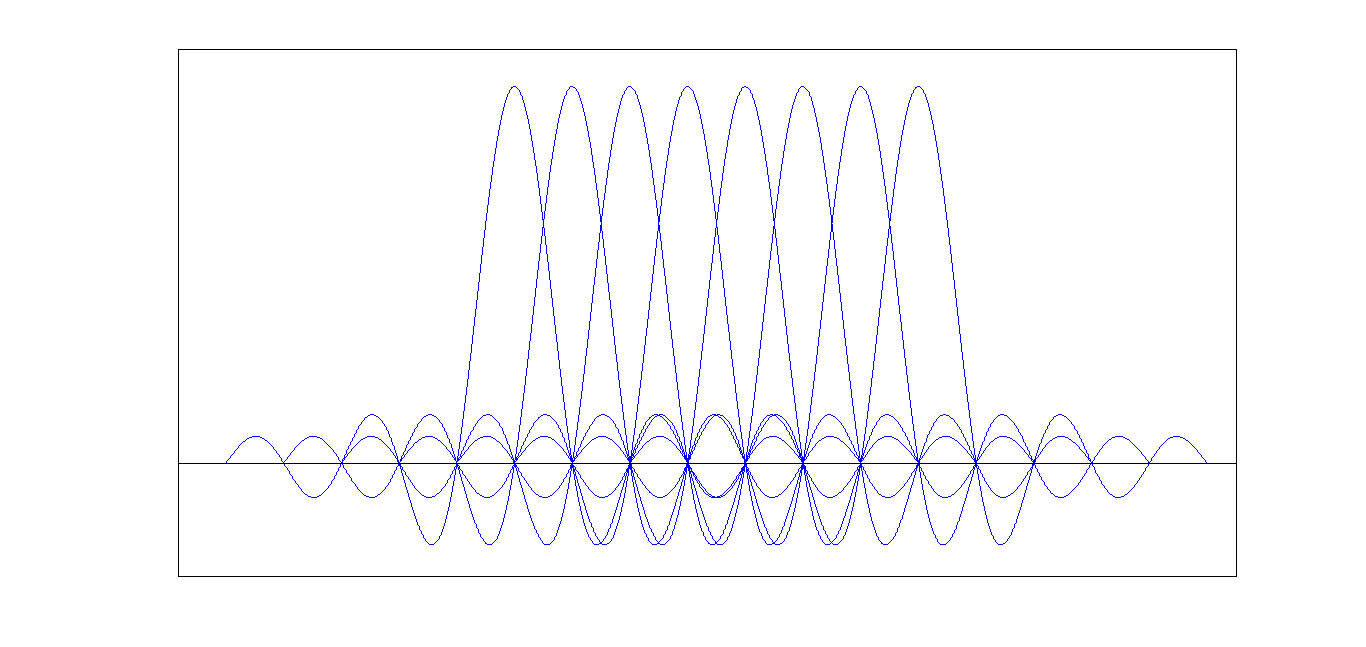
\includegraphics[angle = 0]{./figures/ofdm_subcarriers.png}}
\end{minipage}
\caption{OFDM sub-carriers scheme}
\label{ofdm_carriers}
\end{figure}

The high number of sub-carriers needed to perform a communication at the speeds required nowadays, makes it imposible to be implemented
with dedicated modulators and demodulators for each sub-carrier. The most optimal implementation for the OFDM modulator-demodulator 
is by using Discrete Fourier Transform.\\

The basis of the OFDM transmision is the sum of sub-carriers (wich can be expressed by a complex exponential, or a \textit{frequency}
in the complex plane) multiplied by the data complex symbols. Matematically, it is expressed as seen in equation (\ref{eq:OFDM_symbol_low})

\begin{equation}
s_{k}(t-kT) =
%	\begin{cases}
	w(t-kT) \sum\limits_{i=-N/2}^{N/2-1} x_{i,k} e^{j2\pi
	\left(\frac{i}{T_{FFT}}\right)(t-kT)}
%	\end{cases}
\label{eq:OFDM_symbol_low}
\end{equation}

where \textit{k} is the sub-carrier number. It's easy to recognize in this equation the form of an Inverse Discrete Fourier Transform 
(where the points in the frequency domain are translated to the time domain).\\
Using this, the OFDM modulators bank can be replaced by the computation of a IDFT and the demodulators bank by the computation of a
DFT, making it possible to implement an OFDM modulator/demodulator using a mathemathic computing core. It's even possible to make the 
implementation more optimal by the use of efficient IDFT/DFT algorithms known as Fast Fourier Transform.\\

The objetive of this work is to obtain an FFT computing core, small enough to be included in a complete OFDM transeiver without consuming 
to much resources or space, but efficient enough to be usefull in an ISDB-t television system.

\section{Architechture selection}

There are several algorithms for FFT calculation. Each has some advantages and disadvantages. As we are trying to achieve the smallest
implementation, the radix-r algorithm is selected. It has the particularity of using equal modules in every step of the transform, so
it's the best choice in terms of the implementation efficiency \cite{Schaffer2_3}.\\
Radix-r algorithms are a variation of Cooley-Tukey algorithms \cite{MeyerRadix}. In Cooley-Tukey algorithms the FFT calculation is reduced
to m sub-FFTs through the factorization of the number of points, ($N$). Radix-r variations factorices $N$ in the form of $N = r^\nu$, so the $N$-point FFT 
is decomposed in $\nu$ r-points sub-FFTs. The main advantage of the factorization in $r$ is that the computation module can be replied or reused
for each sub-FFT calculation.\\

\subsection{Radix-r Algorithm}

This algorithm is based in the factorization of the FFT the length $N$ through the bidimentional mapping: 

\begin{equation}
n = N_2n_1 + n_2 \qquad 
	\begin{cases}
	0\leq n_1 \leq N_1 -1 \\
	0\leq n_2 \leq N_2 -1
	\end{cases}
\label{eq:CT_time_inedx}
\end{equation}

\begin{equation}
k = k_1 + N_1k_2 \qquad 
	\begin{cases}
	0\leq k_1 \leq N_1 -1 \\
	0\leq k_2 \leq N_2 -1
	\end{cases}
\label{eq:CT_freq_inedx}
\end{equation}

where $n$ is the time domain index and $k$ is the frequency domain index, and $N=N1*N2$.\\

Expressing the DFT and IDFT in the forms of equations (\ref{eq:DTF}) and (\ref{eq:iDTF})

\begin{equation}
X[k] = \sum_{n=0}^{N-1}x[n]W_N^{kn}
\label{eq:DTF}
\end{equation}

\begin{equation}
x[n] = \frac{1}{N}\sum_{k=0}^{N-1}X[k]W_N^{-kn}
\label{eq:iDTF}
\end{equation}

where $W_N^{kn}=e^{\frac{-j2\pi kn}{N}}$ are known as \textit{twiddle factors}, $n$ and $k$ can be replaced by (\ref{eq:CT_time_inedx})
and (\ref{eq:CT_freq_inedx}):

\begin{equation}
W_N^{kn}=W_N^{N_2n_1k_1+N_1N_2n_1k_2+n_2k_1+N_1n_2k_2} 
\label{eq:Wkn}
\end{equation}

As $W_N^{nk}$ has order $N=N_1N_2$ it becomes that $W_N^{N_1}=W_{N_2}$ and
$W_N^{N_2}=W_{N_1}$, wich replaced in \ref{eq:Wkn}:

\begin{equation}
W_N^{kn}=W_{N_1}^{n_1k_1}W_N^{n_2k_1}W_{N_2}^{n_2k_2} 
\label{eq:Wkn_red}
\end{equation}

Using (\ref{eq:Wkn_red}) in (\ref{eq:DTF}), results in:

\begin{equation}
X[k1,k2]=\sum_{n_2=0}^{N_2-1}
W_{N_2}^{n_2k_2}\left(W_{N}^{n_2k_1}\sum_{n_1=0}^{N_1-1}x[n_1,n_2]W_{N_1}^{n_1k_1}\right)
\label{eq:DFT_mod}
\end{equation}

The inner summation in (\ref{eq:DFT_mod}) is a $N_1$ points DFT multiplied by the factor $W_{N}^{n_2k_1}$. 
Taking $\tilde{x}[n2,k1]=W_{N}^{n_2k_1}\sum_{n_1=0}^{N_1-1}x[n_1,n_2]W_{N_1}^{n_1k_1}$
and replacing in (\ref{eq:DFT_mod}):

\begin{equation}
X[k1,k2]=\sum_{n_2=0}^{N_2-1}
W_{N_2}^{n_2k_2}\tilde{x}[n2,k1]
\label{eq:DFT_tilde}
\end{equation}

(\ref{eq:DFT_tilde}) shows the $N_2$ points $\tilde{x}$ DFT, which represents the main advantage of this algorithm, 
for any factorization of $N$ in the form of $N=N_1N_2$, the $N$ point DFT of $x(n)$ can be calculated following the steps:

\begin{itemize}
  \item Map the input index using (\ref{eq:CT_time_inedx})
  \item Calculate $N_1$ points DFT of $x(n)$.
  \item Multiplie the resulting points by the twiddle factors.
  \item Calculate $N_2$ point DFT of the resulting secuence.
  \item Map the output index using (\ref{eq:CT_freq_inedx})
\end{itemize}

Here we can subdivide the sub-DFTs applying the described method in turn to reduce the original DFT to 
several sub-DFTs of smaller length and simpler to operate.

An extra advantage of this algorithm is the posibility of in-place memory using, where the results of an operation
is holded in the memory position of the operands, so for a $N$ point DFT needs a $N$ length memory.

Radix-r is a variation of this algorithm where $N=r^\nu$. The value of $r$ affects the type of operations needed by the algorithm, as can
be seen in table \ref{table:fft_oper}.

\begin{table}[h]
\begin{tabular}{c c c c}
\textbf{r} & \textbf{Multiplications} & \textbf{Non trivial multiplications} &
\textbf{additions} \\ \hline 
$2$ & $2$ & $0$ & $2$ \\
$3$ & $3$ & $2$ & $6$ \\
$4$ & $4$ & $0$ & $8$ \\
$5$ & $6$ & $5$ & $17$ \\
$7$ & $9$ & $8$ & $36$ \\
$8$ & $8$ & $2$ & $26$ \\
$9$ & $11$ & $10$ & $44$ \\ \hline
\end{tabular}
\caption{Complex operations quantity for different values of \textit{r}}
\label{table:fft_oper}
\end{table}
 
For $r=2$ and $r=4$ there aren't any non trivial multiplications, so this are the values chosen for $r$.\\
A radix-r FFT has $log_rN$ stages. As table \ref{table:fft_oper} shows, for $r=4$ more operations per stage are needed but there are
half the stages. Both are implemented in order to make a comparition between them and provide the posibility to choose
depending on the requirements of the implementation.

\subsection{Implementation of the Radix-r architechture}

Figure \ref{fig:r2_8} shows the simplified scheme of an $8$ points radix-2 FFT.

\begin{figure}[htb!]
        \centering
        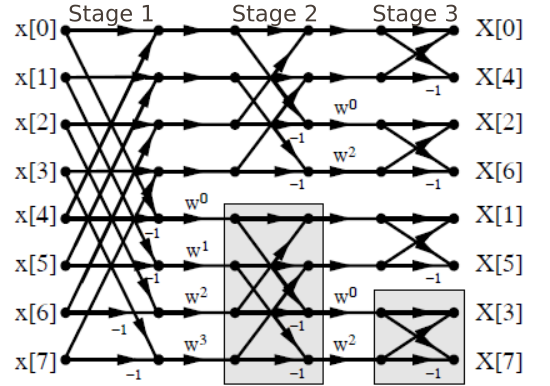
\includegraphics[width=7cm]{./figures/r2_8.png}
        \caption{8 points Radix-2 FFT}
        \label{fig:r2_8}
\end{figure}

Each node represents an addition and the arrows represents the multiplication by the value over the arrow. 
The figure shows the stage division of the algorithm, each one performs a $2$ points DFT. Each $2$ points DFT 
is known as a Butterfly. For a radix-4 DFT, the scheme is similar but every node is a four points addition.\\
In general, for a $N$ points DFT $\frac{N}{2}*\log_2(N)$ butterflies and $\frac{N}{2}*(\log_2(N)-1)$ complex multipliers
are needed. But there are alternative implementations for the radix algorithms wich provides optimizations in 
butterflies and multipliers quantity, memory length, throughput (related with the transmition speed) and control-unit
complexity.\\
The most-common implementations are:

\begin{itemize}
  \item \textbf{Parallel} All \textit{butterfly} and multipliers are implemented in similar scheme as 
  the one showed in \ref{fig:r2_8}.
  \item \textbf{Unrolled} Single Delay Feedback (SDF) architechture \cite{torkelson}. 
  Figure \ref{fig:r2sdf} shows a $4$ point radix-2 SDF FFT scheme.
  It uses a \textit{butterfly} and a complex multiplier per stage.
  \item \textbf{Iterative} It implements only one \textit{butterfly} and one complex multiplier, wich performs secuencially
  the operation for every stages. Figura \ref{fig:r2sBf} shows a $8$ points iterative radix-2 FFT scheme. 
\end{itemize}

\begin{figure}[htb!]
        \centering
        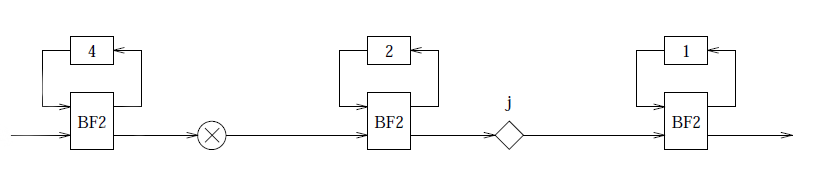
\includegraphics[width=9cm]{./figures/r2sdf.png}
        \caption{Unrolled SDF Radix-2}
        \label{fig:r2sdf}
\end{figure}

\begin{figure}[htb!]
        \centering
        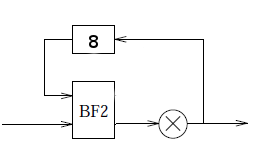
\includegraphics[width=6cm]{./figures/r2sBf.png}
        \caption{Iterative Radix-2}
        \label{fig:r2sBf}
\end{figure}

Table (\ref{table:radixcomp}) shows the comparision of characteristics of the three implementations descrived above.

\begin{table}[htb!]
\centering
\begin{tabular}{l c c c}
\textbf{Characteristic} & \textbf{Parallel} & \textbf{Unrolled} &
\textbf{Iterative}\\
\hline 
\# \textit{butterfly} & $\frac{N}{\nu}*\log_\nu(N)$ & $\log_\nu(N)$ & $1$ \\
\# multipliers & $\frac{N}{\nu}*(\log_\nu(N)-1)$ & $log_\nu(N)-1$ & $1$ \\
Memory length & $0$ & $N-1$ & $N$ \\
Bus type & Parallel & Serie & Serie \\
\textit{throughput} & $N$ points per cicle & $1$ point per cicle & $1$ per $\log_\nu(N)$
cicles\\
\textit{pipeline} & Yes & Yes & No\\
\hline
\end{tabular}
\caption{Comparative between parallel, unrolled and iterative radix-r}
\label{table:radixcomp}
\end{table}

One restriction of the implementation is the space efficiency, so the iterative implementation is selected, because it only needs
one butterfly and one multiplier independently of FFT length. In terms of space, the relation between the iterative vs the unrolled 
efficiency is $log_r(N):1$ Only the memory size depends on FFT length, but it is equal to the 
unrolled implementation, so there no advantages. This ensures the low space and low energy needed by the core.\\
Even though it represents low throughput, it is easily solved by feeding the core clock with the correct frequency.\\

\subsection{Twiddle factors multiplication}

Radix algorithms require the multiplication by twiddle factors. Is well known that multiplications in digital implementation are worthy, 
spacial and temporaly. So to choose the better alternative needs a carefully analisys.\\

Three methods were analised:
\begin{itemize}
  \item Cordic Algorithm
  \item BKM Algorithm
  \item Efficient complex multiplication
\end{itemize}

\subsubsection{Cordic Algorithm}

Twiddle factors have the form $W_N^{kn}=e^{\frac{-j2\pi kn}{N}}$. So in the complex axis they represent a rotation. A well known and well proved 
algorithm for rotations is the cordic algorithm. It is based on successive aproximations by micro-rotations until the desired angle is reached.\\
The algorithm is defined by the following rotation equations:

\begin{equation}
x_{i+1} = x_i* \cos \theta_{i+1} - y_i* \sin \theta_{i+1}
\label{eq:micrototX}
\end{equation}

\begin{equation}
y_{i+1} = y_i* \cos \theta_{i+1} + x_i* \sin \theta_{i+1}
\label{eq:micrototY}
\end{equation}

The main advantage of this algorithm is that it only uses additions (and substractions) and shifts, both of them very cheap in terms \\
of resources. Also it can be pipelined, improving the speed of processing.\\

For more details of Cordic Algorith refer to \cite{Volder}.

\subsubsection{BKM Algorithm}

This algorithm, like the cordic algorithm, try to resolve elemental equations using only additions and shifts.\\
It is based on the following equations:

\begin{equation}
	\begin{cases}
	L_{n+1} = L_n(1+d_n*2^{-n}) \\
	E_{n+1} = E_n - \ln (1+d_n*2^{-n})
	\end{cases}
\label{eq:BKM}
\end{equation}

In comparition with Cordic Algorithm, BKM requires more storage and is more complex. In addition, it's main efficience is obtained using 
redundant numeric system. In the case of this work, the implementation is made usign two's complement number representation, wich is not redundant.\\
Because of this reasons, BKM is discarded for this project. For more information about BKM algorithms refer to \cite{BKM}.

\subsubsection{Efficient Complex multiplier}

Cordic algorithm is widely used in FFT calculation because of its very low cost in terms of space and resources. But in an iterative 
implementation, where only one multiplier is required, the difference between the cordic core and a complex multiplier is very little.\\

For twiddle factors, the multiplication required is:

\begin{equation}
R+jI = (A+jB)*(C+jD) = (A*C-B*D) + j(A*D+B*C)
\label{eq:prodcomp4}
\end{equation}

where $(C+iD)$ is the twiddle factor. A straight implementation would need four multipliers, but pre-calculating some of the factors and 
storing them in memory (as the $tg\theta$ in cordic) can reduce the implementation to only three multiplications, in fact, a $25 \%$.\\

Pre-calculated factors are $C$, $(C+D)$ and $C-D$. Then, getting into the multiplier with the twiddle factor, pre-calculated values 
are used to obtain $Z = C x (A-B)$ and then:

\begin{equation}
R = (C-D) \times B + Z
\label{eq:prodcompR}
\end{equation}

\begin{equation}
I = (C+D) \times A - Z
\label{eq:prodcompI}
\end{equation}
 
Taking into account that several FPGAs have DSP integrated modules, the implementation of multipliers could be very efficient.\\

\subsection{Summary of implementation}

As it has been exposed in this section, the following architechtures are implemented:

\begin{itemize}
  \item Radix-2 iterative architechture.
  \item Radix-4 iterative architechture.
  \item Cordic algorithm for twiddle factors multiplications, for radix-2 and radix-4.
  \item Efficient complex multiplier for twiddel factors multiplications, for radix-2 and radix-4, as an alternative to 
  cordic algorithm.
\end{itemize} 

\section{Radix-2}

As it has been explained in previous sections, an iterative implementation for the N points radix-2 algorithm uses only one butterfly 
for the calculations fo every stage consecutevely. This ledas to waitng $log_2(N)$ cicles between two entry point and between two output points.\\
In Figure (\ref{fig:r2_8}) are shown the different stages of radix-2 FFT implementation.\\
On each clock cicle, one of two posible operations can be performed:

\begin{itemize}
  \item A point is stored in memory while another point is sended from memory to twiddle factor multiplier or to the core output.
  \item A butterfly operation between a core-input point or last-stage point and a memory-stored point. Two points results from the
  butterfly operation: one is stored in memory while the other is sended to the twiddle factor multiplier or to the output.  
\end{itemize}

%Figure (\ref{fig:radix2blocks}) provides a block diagram for radix-2 iterative implementation. There can be apreciated the main components 
Main components of the core are: N point memory, butterfly, multiplier an dthe control unit. an input ultiplexer determines if the 
butterfly operation will be done with the core entry point or with a point stored in memory.\\

% \begin{figure}[htb!]
%         \centering
%         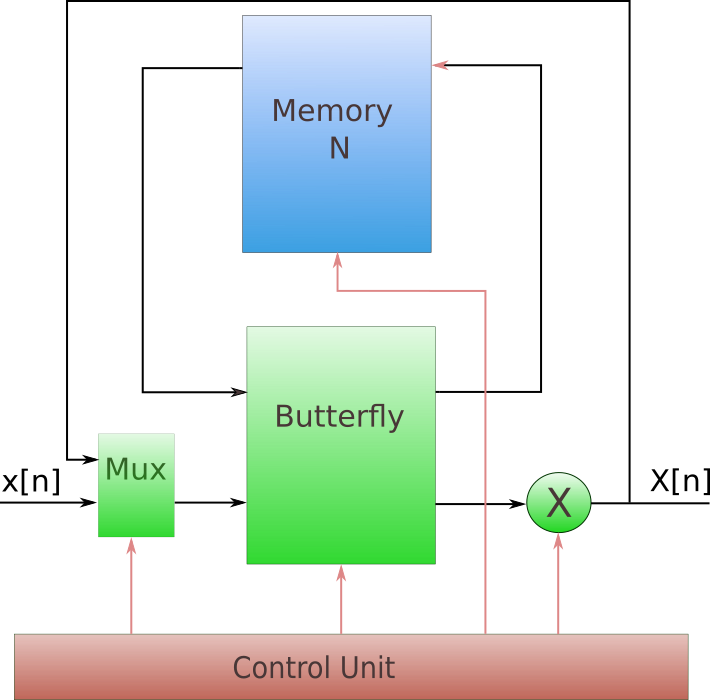
\includegraphics[width=6cm]{./figures/radix2blocks.png}
%         \caption{Iterative radix-2 simplified diagram}
%         \label{fig:radix2blocks}
% \end{figure} 

\subsection{Memory}

Due to the type of memory operations, simultaneous store and read data, the memory unit is implemented as a two-port RAM memory of length N. 
In fact, there is only $N-1$ memory positions needed, but for ease a N memory is implemented, because there is always one point from a stage that is used in 
the next stage, so it has not to be stored in memory. Memory positions have 2 word length in order to store the real and imaginary part of every point.

\subsection{Butterfly}

The butterfly unit has to perform the two operands complex operations:

\begin{equation}
\begin{split}
c &= a+b \\
d &= a-b
\end{split}
\label{eq:butterf}
\end{equation}

\subsection{Datapath}

The datapath must comprise both types of operations described above, and trhee different variants for eacg one: the incoming data for a given stage could
come from the core input or from the previous stage and/or from the memory, and the resulting data could go to the core output or to the
multiplier and/or to the memory.\\
When a memory-store operation is performed, a cero ('0') is added or substracted to the operand so it is stored in memory through the 
butterfly unit.\\
This is done by a set of multiplexers controlled by the control unit.   

\subsection{Control Unit}

The control unit has to set the multiplexers according to the operation that is performed in that clock cicle, address the memory to the 
position wherer the actual operand has to be readed or stored and generate the twiddle factors for the multiplier.\\
Given that the core has $log_2(N)$ stages, the control unit has a stage-counter with length $log_2(log_2(N))$. Another counter, with a
length of $log_2(N)$ counts the number of points that have entered into the core by that moment. A state machine is controlled with 
these counters. Is this state machine the one wich controlls the architechture.\\

To decide if a particular stage performs an arithmetihci or a memory transfer operation, a bit of the points counter is evaluated. 
The position of that bit is determined by the stage counter, as shown in Figure (\ref{fig:r2conts}) for an 8 point radix-2.

\begin{figure}[htb!]
        \centering
        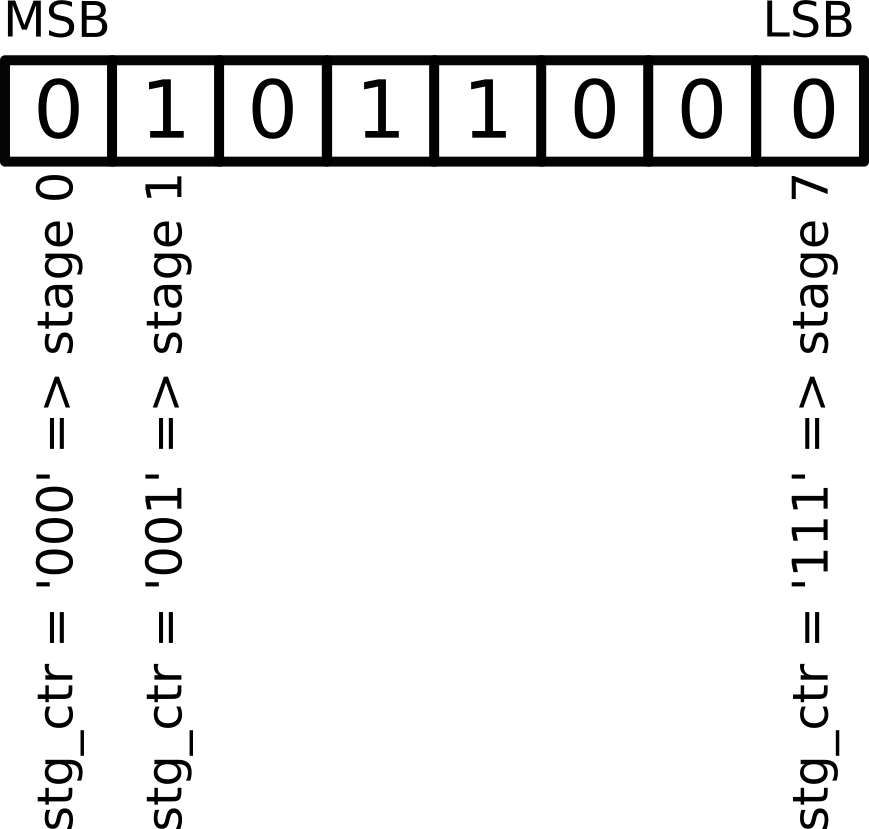
\includegraphics[width=3cm]{./figures/r2conts.png}
        \caption{Point counter bit selection}
        \label{fig:r2conts}
\end{figure} 

Memory control is doing by the reading and writing addresses and the read and write control signals. As in this case the memory is readed 
and writed in every clock cicles, control signals are always asserted. Respecting the addressing, being the radix-2 an in-place storing
algorithm, in every clock cicle the result of an operation is stored in the same memory position of one of its operands. So the reading 
address and the writting address are the same, and corresponds to the points counter value.

\subsection{Integration}

Figure (\ref{fig:datapathmem}) presents the integrated core. Control unit signal are shown as arrows to keep the graphic clear.\\
An additional register is placed before the multiplier because one result of a given stage is used in the following stage, so
it must be keeped for one clock cicle. Another register is placed in the output in order to bring secuencial sinchronization 
with the circuit connected to the core.\\
An optional scaling unit is provided after the butterfly to give a method to deal with overflow. The scaling unit can be turned on 
selectivelly for each stage in real time. 

\begin{figure}[htb!]
        \centering
        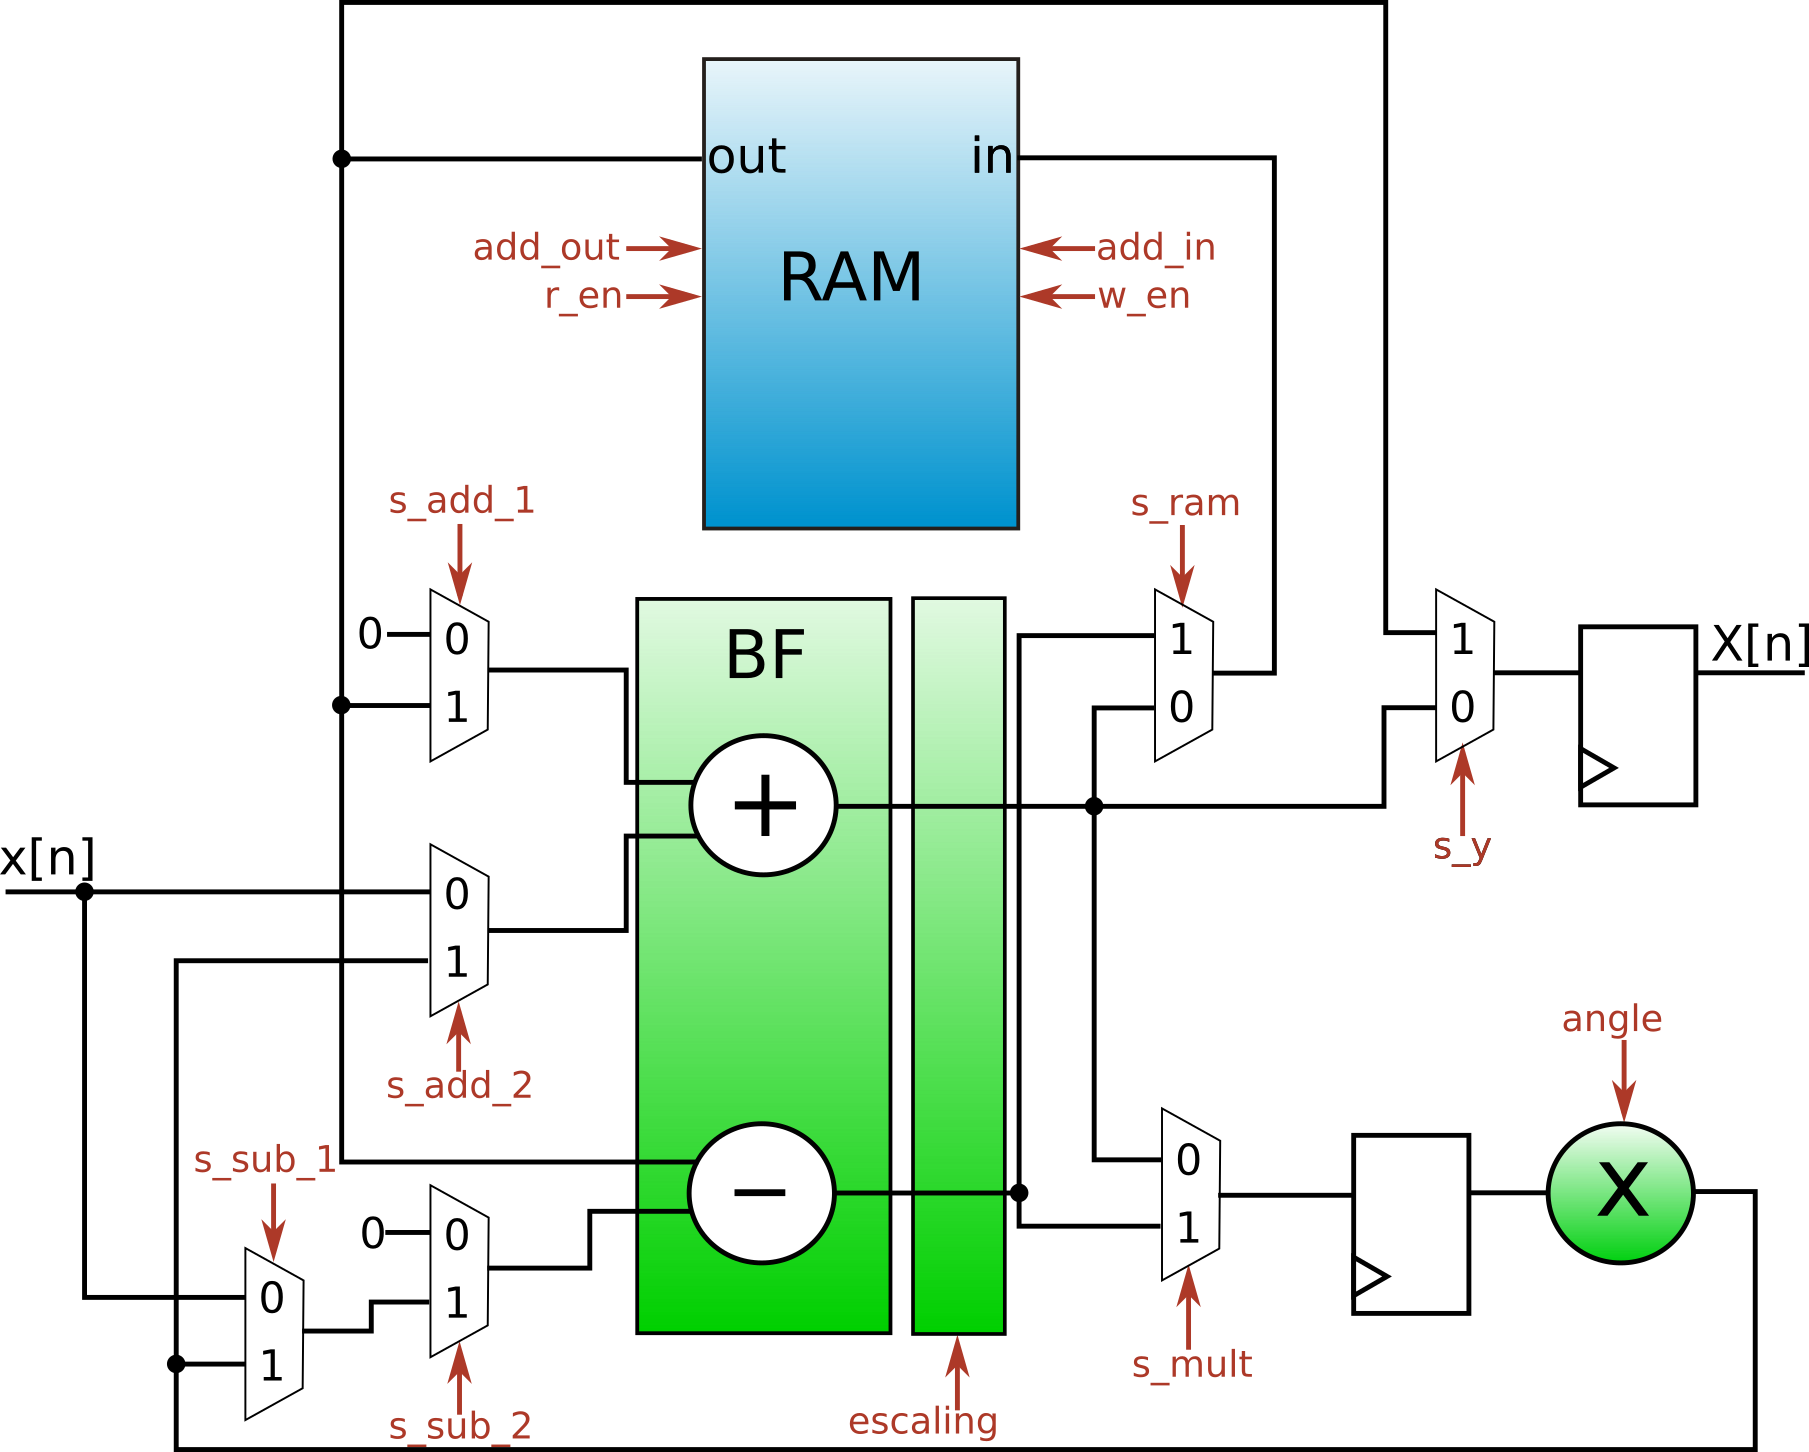
\includegraphics[width=9cm]{./figures/datapathMem.png}
        \caption{Datapath with control signals}
        \label{fig:datapathmem}
\end{figure}
 
\section{Radix-4}

Radix-4 algorithm divides a N-point DFT in $\nu$ 4-point DFT, so that $N = 4^\nu$.\\
Breaking up the N-point DFT in 4 DFT of $N/4$ points each, it becomes to the next four expressions 
wich resumes the operations the radix-4 has to process (\cite{MeyerRadix}):

\begin{equation}
y_n = (x_n + x_{n+\frac{l}{4}} + x_{n+\frac{l}{2}} + x_{n+\frac{3l}{4}})
\label{eq:radix4_suby}
\end{equation}

\begin{equation}
z_n = ((x_n - x_{n+\frac{l}{2}}) -j (x_{n+\frac{l}{4}}
-x_{n+\frac{3l}{4}})) W_N^{k}
\label{eq:radix4_subz}
\end{equation}

\begin{equation}
g_n = ((x_n + x_{n+\frac{l}{2}}) - (x_{n+\frac{l}{4}}
+ x_{n+\frac{3l}{4}})) W_N^{2k}
\label{eq:radix4_subg}
\end{equation}

\begin{equation}
h_n = ((x_n - x_{n+\frac{l}{2}}) +j (x_{n+\frac{l}{4}} - x_{n+\frac{3l}{4}})) W_N^{3k}
\label{eq:radix4_subh}
\end{equation}

for $k = 0,1,\ldots,\frac{N}{4}-1$, where $l$ depends on the current processing stage:

\begin{equation}
\begin{split}
l_1 &= N \\
l_2 &= \log_4(N) \\
l_3 &= \log_4(\log_4(N)) \ldots\\
l_\nu &= 4
\end{split}
\label{eq:radix_4_arit_l}
\end{equation}

where $l_i$ corresponds to the i-ith stage of a $N=4^\nu$ point DFT.

It's clear that the radix-4 algorithm must process four points in each arithmetic operation: $x_n$,
$x_{n+\frac{l}{4}}$, $x_{n+\frac{l}{2}}$ and $x_{n+\frac{l}{4}}$.

Figure (\ref{fig:r4_diag})shows the operatinal scheme of a 16-points radix-4 algorithm.

\begin{figure}[htb!]
        \centering
        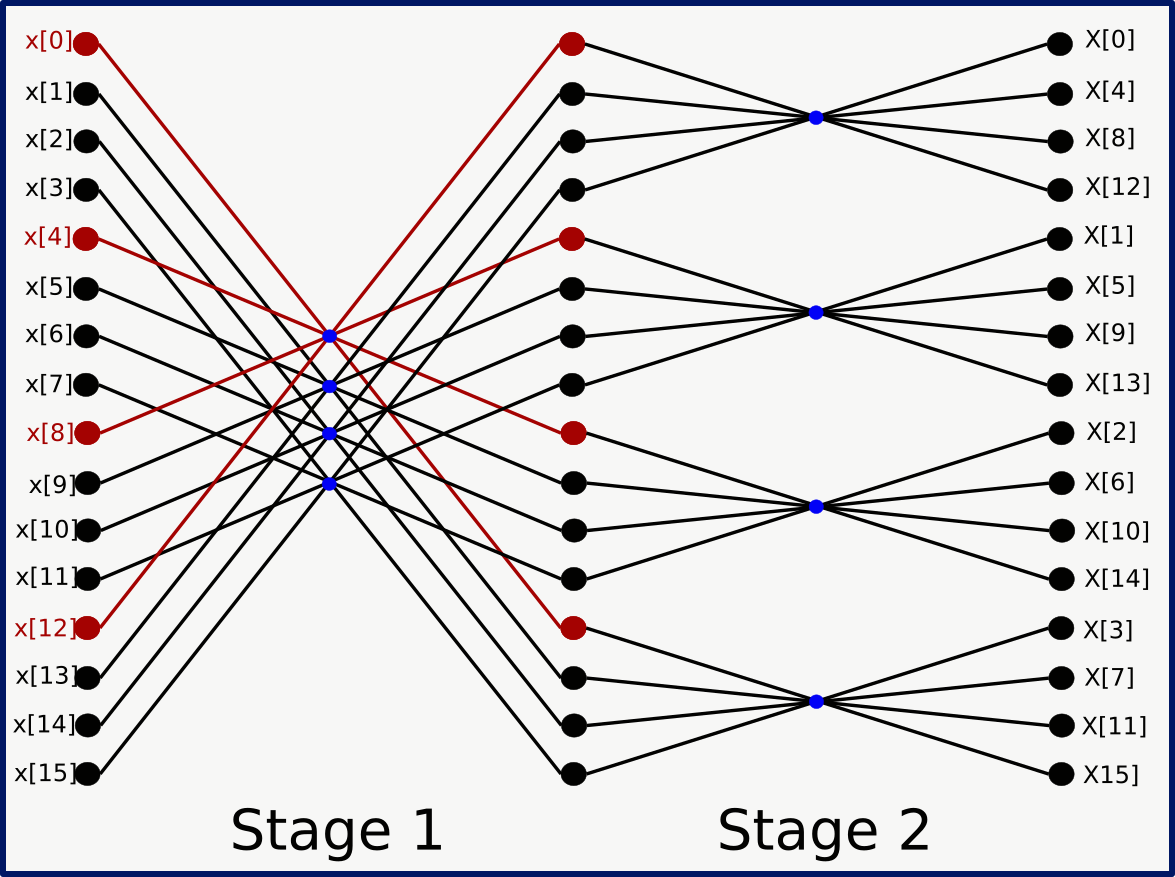
\includegraphics[width=7cm]{./figures/r4_16.png}
        \caption{16 points Radix-4 FFT diagram}
        \label{fig:r4_diag}
\end{figure}

On each clock cicle, one of four posible operations is performed:

\begin{itemize}
  \item A point is stored in memory sub-block A, from the twiddle factor multiplier, while another point is sended from memory 
  sub-block A to the multiplier or the output.
  \item B point is stored in memory sub-block B, from the twiddle factor multiplier, while another point is sended from memory 
  sub-block B to the multiplier or the output.
  \item C point is stored in memory sub-block C, from the twiddle factor multiplier, while another point is sended from memory 
  sub-block C to the multiplier or the output.
  \item An arithmetic operation is performed with a point from the core input or the previous stage and 3 points from memory, each
  from a different memory sub-block. 
\end{itemize}

It can be appreciated that each arithmetic operation needs 4 operands, one will come from the core input or the previous stage and the other
3 will come from the storage memory, so a special memory is designed for this implementation.\\
Again, the main components are the memory, the aritmetic unit (called dragonfly), the datapath and the control unit.

\subsection{Memory}

As saying above, artihmetic operations needs 3 operands from memory, so a 3-way in 3-way out memory is needed. 
In order to take advantage of the memory blocks present 
in most FPGAs, a special memory is designed for this core, formed by 3 dual-port RAMs similar to radix-2 memories. This way, 
in each arithmetic operation, an operand of each memory sub-block can be readed and stored simultaneously.\\
As the directions may not be succesive, because in each clock cicle a different stage operation is performed, each sub block 
is divided in $\nu$ regions delimited by the address. Sub-block address regions are showed in Figure (\ref{fig:tripleRamdir}).

\begin{figure}[htb!]
        \centering
        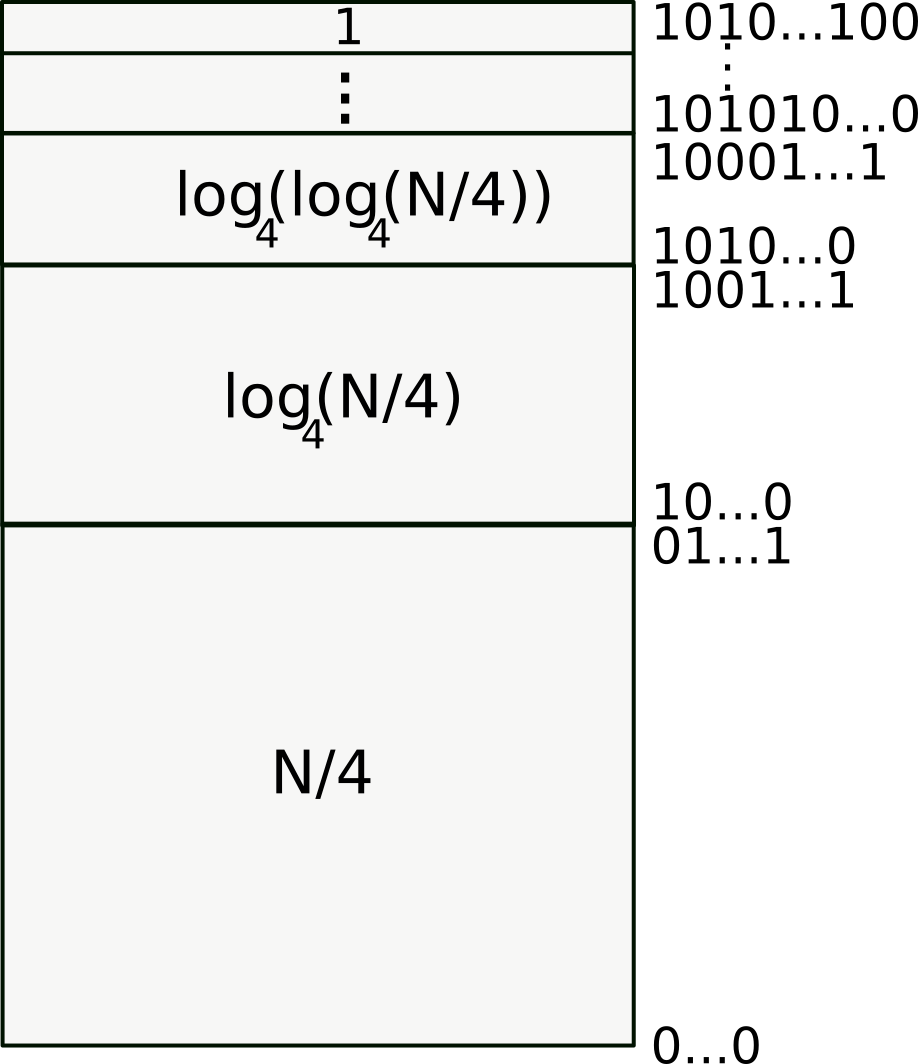
\includegraphics[width=4cm]{./figures/tripleRAMdir.png}
        \caption{Memory sub-blck addressing map}
        \label{fig:tripleRamdir}
\end{figure} 
 
 \subsection{Dragonfly}
 
 The arithmetic unit performs the equations (\ref{eq:radix4_suby}) to (\ref{eq:radix4_subh}), wich are directly implemented in 
 the logic.\\
 In each stage two different types of operations can be performed: a four point arithmetic calculation or a memory data traslation.
 In the last case, a point from a memory sub-block is trasferred to the multiplier, while a point is stored in the next stage memory sub-block.
 The dragonfly unit includes an inner datapath wich guides the data according to the operation in progress.\\
 A block diagram of the arithmetic is presented in Figure (\ref{fig:firefly}). 
 
 \begin{figure}[htb!]
        \centering
        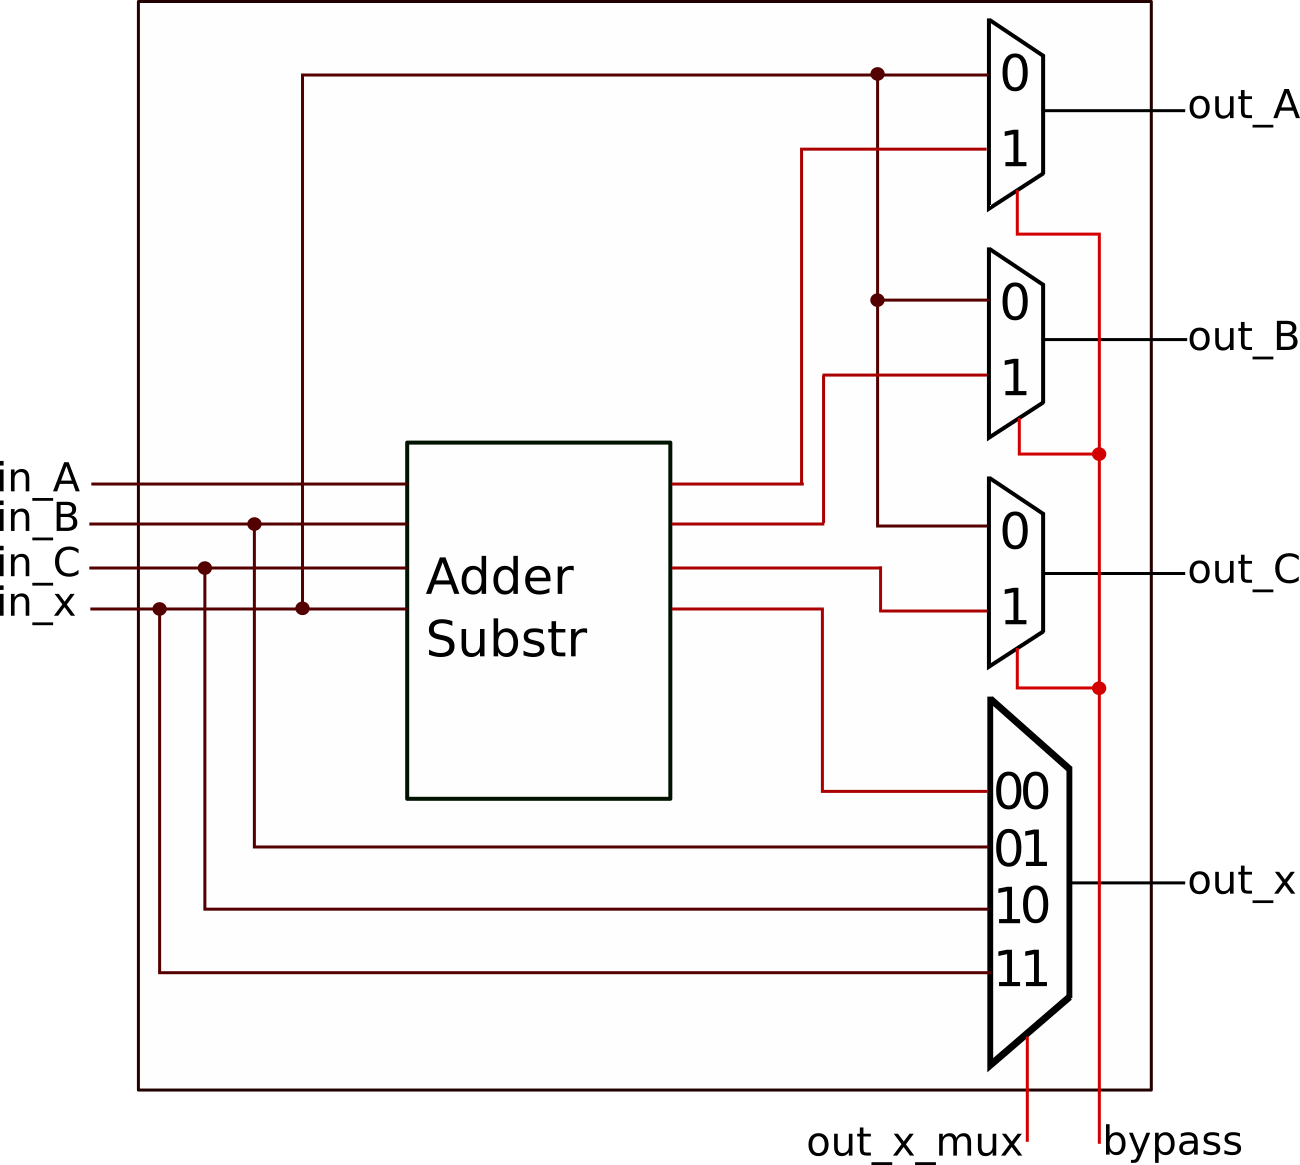
\includegraphics[width=6cm]{./figures/firefly.png}
        \caption{Arithmetic unit block diagram}
        \label{fig:firefly}
\end{figure}
 
 \subsection{Datapath}
 
 The datapath must comprise both types of operations (memory transfer are in fact three different operations as it can be done from and to 
 one of the three memory sub-blocks). The design schem is similar to radix-2 datapath, leaving the sub-block selection path to the
 dragonfly inner datapath. 
 
 \subsection{Control unit}
 
 As well as in radix-2, the control unit configures the datapath and generate the memory addresses and the twiddle factors for
 the multiplier. But in this case, a new point arrives every $log_4(N)$ clock cicles, while in radix-2 it occurs every $log_2(N)$, 
 wich determines the stage number.\\
 Also, two counters as used: a $log_2(N)$ length points counter and a $log_2(log_4(N))$ length stage counter. Determination of wich operation
 must be perform in a giiven clock cicle is done by the evaluation of pair of bits fo the point counter refered by the value of 
 the stage counter, as shown in Figure (\ref{fig:r4conts}).
 
 \begin{figure}[htb!]
        \centering
        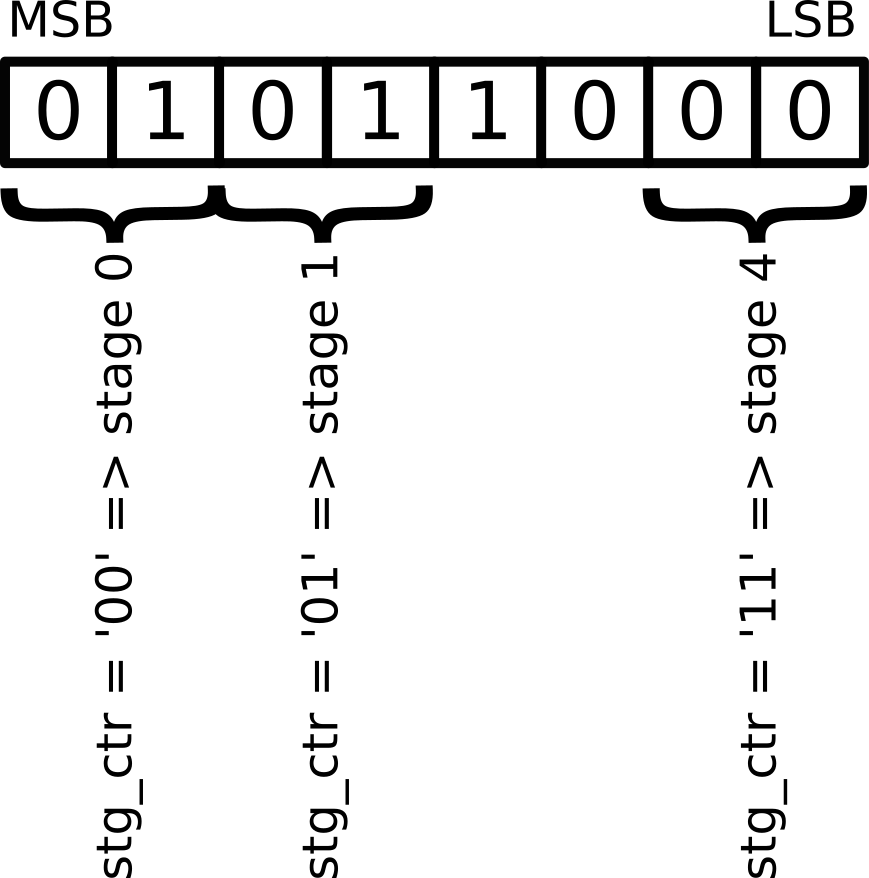
\includegraphics[width=4cm]{./figures/r4conts.png}
        \caption{Point counter bits for operation selection}
        \label{fig:r4conts}
\end{figure}   

Memory addressing is done mapping directly the point counter to the memory addresses. The sub-block region selecetion is done using the 
stage counter because each sub-block is subdivided in regions for each stage. The read and write control signalas are controlled according 
to the type of operation: in memory transfer operations only the correct sub-block is enabled, in arithmetical operations all three sub-blocks
are allowed to be readed and writed.

\subsection{Integration}

Figure (\ref{fig:datapathR4control}) presents the iterative radix-4 core. As in radix-2, extra registers are added after arithmetic unit and in 
the output. A rounding/clipping unit is added to the dragonfly ti prevent overflow.  

\begin{figure}[htb!]
        \centering
        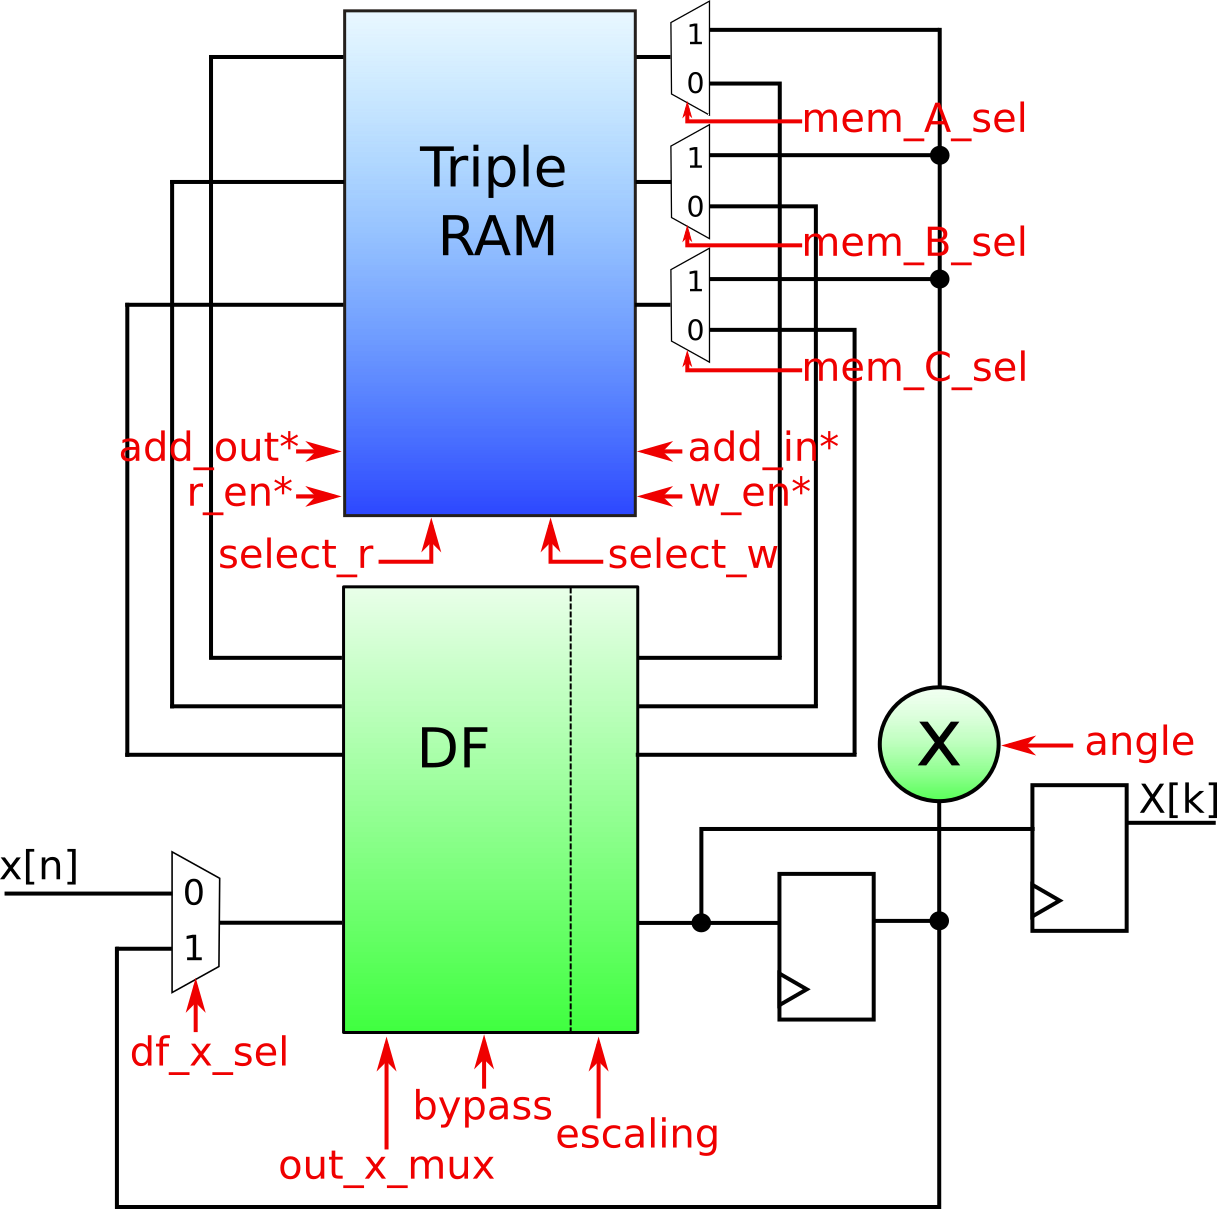
\includegraphics[width=7cm]{./figures/datapathR4control.png}
        \caption{Datapath with control signals}
        \label{fig:datapathR4control}
\end{figure} 
 
\section{Architecture Characterization}

Beside of the individual tests for every composing unit, a set of tests is made over the entire architectures in order to verificate and validate the design.\\
For a complete description of tests and results, refer to \cite{tesis}.

\subsection{Standard signals}
First, a set of standard signals is applyed to the cores, and the result is compared to the expected result. The cores are 
configurated in IFFT mode.
The signals are:

\begin{itemize}
  \item Delta in frequency component '0'. Expected a continuous signal.
  \item Delta in frequency component 6. Expected six cicles of a sin.
  \item Sin of period N/6. Expected a delta in time component 6.
\end{itemize}

All the tests were passed correctly.

\subsection{Error measurement}

In order to measure the architecture error, Matlab fft is taken as a benchmark because it operates with 64 bits floating point numbers,
wich is mpre accurate than 12 or 16 bits integer numbers of the cores.\\

Two metrics are used for error measuring, $E_\infty$ and $E_2$:

\begin{equation}
E_\infty = MAX(\frac{ X_o[n] - X_{dut}[n]}{X_o[n]})
\label{eq:norma1}
\end{equation}

\begin{equation}
E_2 = \Vert\frac{X_o[n] - X_{dut}[n]}{X_o[n]}\Vert_2
\label{eq:norma2}
\end{equation}
 
It's important to note that the radix architectures are non lineal, so for solving this, every test consists of $1024$ simulations with random vector inputs.
In each simulation, the result of the core computation is compared with Matlab result and the errors are compupted. After the $1024$ simulations, 
error values are promediated to obtain the final error values.\\
This is done for $12$ and $16$ bit implementation aof radix-2 and radix-4 cores. This is because $12$ bits is a standard word length in OFDM comunication systems 
and $16$ bits is a standard in signal processing. Also cordic and complex multiplier versions are tested, in order to comparate their performance.\\
As an extra test bench, a widely used, 16 bit integer C++ FFT core is tested \cite{KISSFFT}.

\begin{table}[htb!]
\begin{tabular}{l c c c c}
 & \textbf{1024, 12 bits} & \textbf{1024, 16 bits} & \textbf{4096, 12 bits} & \textbf{4096, 16 bits}\\ \hline 
\textbf{Radix-2, Cordic} & $0.092$ & $0.006$ & $0.099$ & $0.008 $\\
\textbf{Radix-2, Mult.} & $0.232$ & $0.003$ & $0.340$ & $0.108$\\
\textbf{Radix-4, Cordic} & $0.077$ & $0.003$ & $0.074$ & $0.007$\\
\textbf{Radix-4, Mult.} & $0.224$ & $0.002$ & $0.334$ & $0.105$\\
\textbf{Kiss FFT} & $ $ & $0.017$ & $ $ & $0.035$\\\hline
\end{tabular}
\caption{$E_\infty$ for 1024 simulations with random inputs}
\label{table:errorInf}
\end{table}

\begin{table}[htb!]
\begin{tabular}{l c c c c }
 & \textbf{1024, 12 bits} & \textbf{1024, 16 bits} & \textbf{4096, 12 bits} & \textbf{4096, 16 bits}\\ \hline 
\textbf{Radix-2, Cordic} & $0.095$ & $0.007$ & $0.116$ & $0.053$\\
\textbf{Radix-2, Mult.} & $0.257$ & $0.004$ & $0.356$ & $0.131$\\
\textbf{Radix-4, Cordic} & $0.084$ & $0.002$ & $0.094$ & $0.027$\\
\textbf{Radix-4, Mult.} & $0.258$ & $0.003$ & $0.358$ & $0.126$\\ 
\textbf{Kiss FFT} & $ $ & $0.017$ & $ $ & $0.035$\\\hline
\end{tabular}
\caption{$E_2$ for 1024 simulations with random inputs}
\label{table:error2}
\end{table}
 
In tables \ref{table:errorInf} and \ref{table:error2} is clear that performance of the cores is perfectly suitable for OFDM systems. Moreover, 
the cores can be used in signal processing as the error is under 1\%. For complex multiplier the error can be cutted down by increasing the word 
length of the factors stored in memory. For Cordic rotator, the error can be cutted down by adding rotation steps.\\

\subsection{THD}

In order to measure the THD of the architectures, $16$ test are performed. One for each architecture, radix-2 or radix-4, for all flavours 
described before: $12$ or $16$ bits, $1024$ or $4096$ points and cordic or complex multiplier for twiddle factors. Additionally, THD test is made 
over KISFFT to get a testbench.\\
Each test run consecutive simulations using as input a tone in every input point each time. That way, a graphic can be made with 
the armonic response to every frequency tone. Figures (\ref{fig:r2_thd_1024_com}) to (\ref{fig:r4_thd_1024_cor}) shows some of the 
resulting graphics.\\
That graphics shows that the core response is similar as the KISSFFT response and also as the Matlab FFT response. So the THD 
is perfectly acecptable.

\begin{figure}[Htb!]
        \centering
        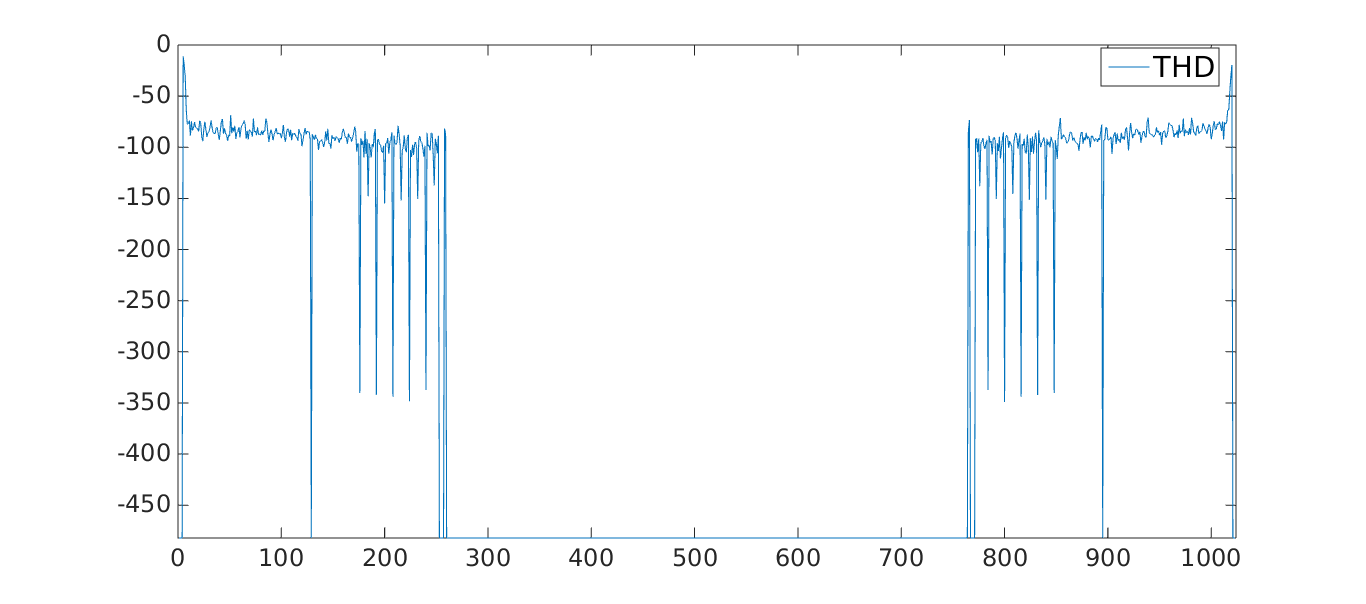
\includegraphics[width=7cm]{./figures/thd_r2_1024_12_mul.png}
        \caption{R-2, complex mult., 12 bits}
        \label{fig:r2_thd_1024_com}
\end{figure}

\begin{figure}[Htb!]
        \centering
        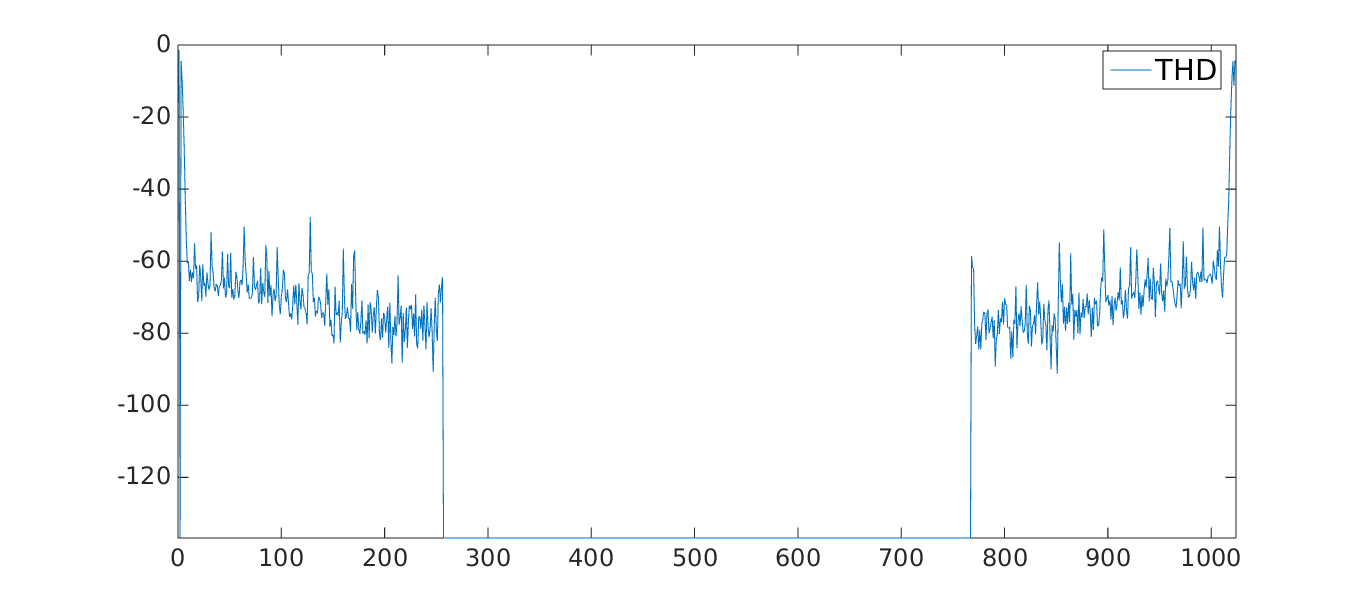
\includegraphics[width=7cm]{./figures/thd_r2_1024_12_cor.png}
        \caption{R-2, Cordic, 12 bits}
        \label{fig:r2_thd_1024_cor}
\end{figure}

\begin{figure}[Htb!]
        \centering
        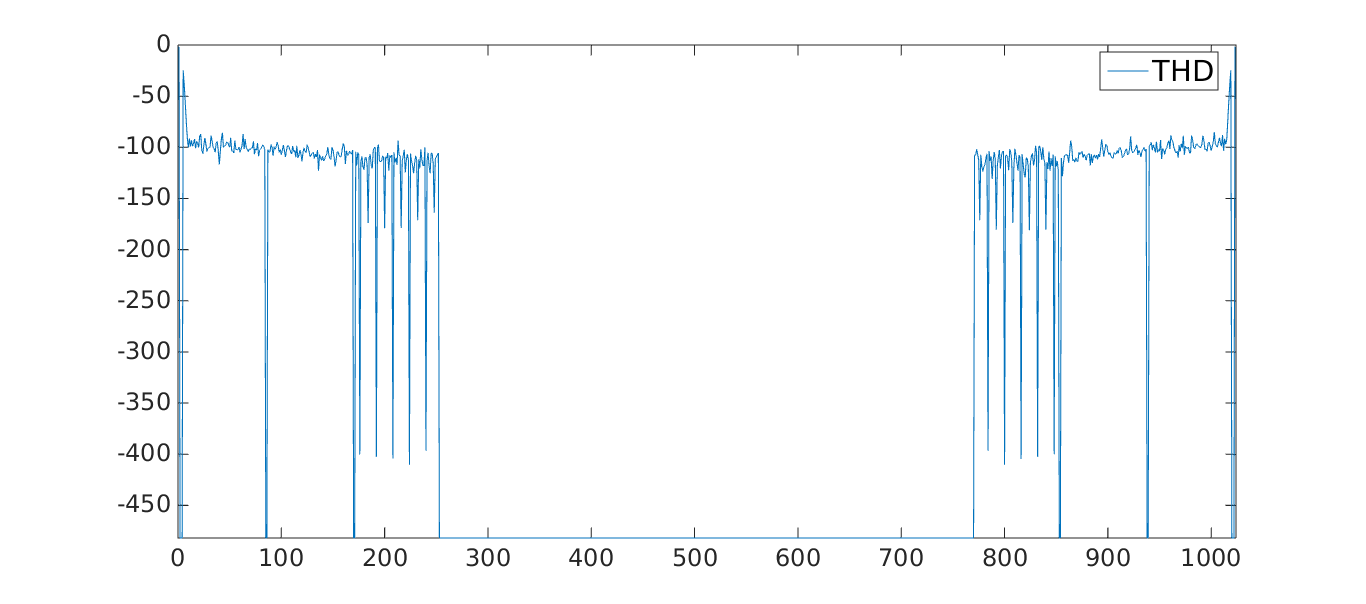
\includegraphics[width=7cm]{./figures/thd_r4_1024_12_mul.png}
        \caption{R-4, complex mult., 12 bits}
        \label{fig:r4_thd_1024_com}
\end{figure}

\begin{figure}[Htb!]
        \centering
        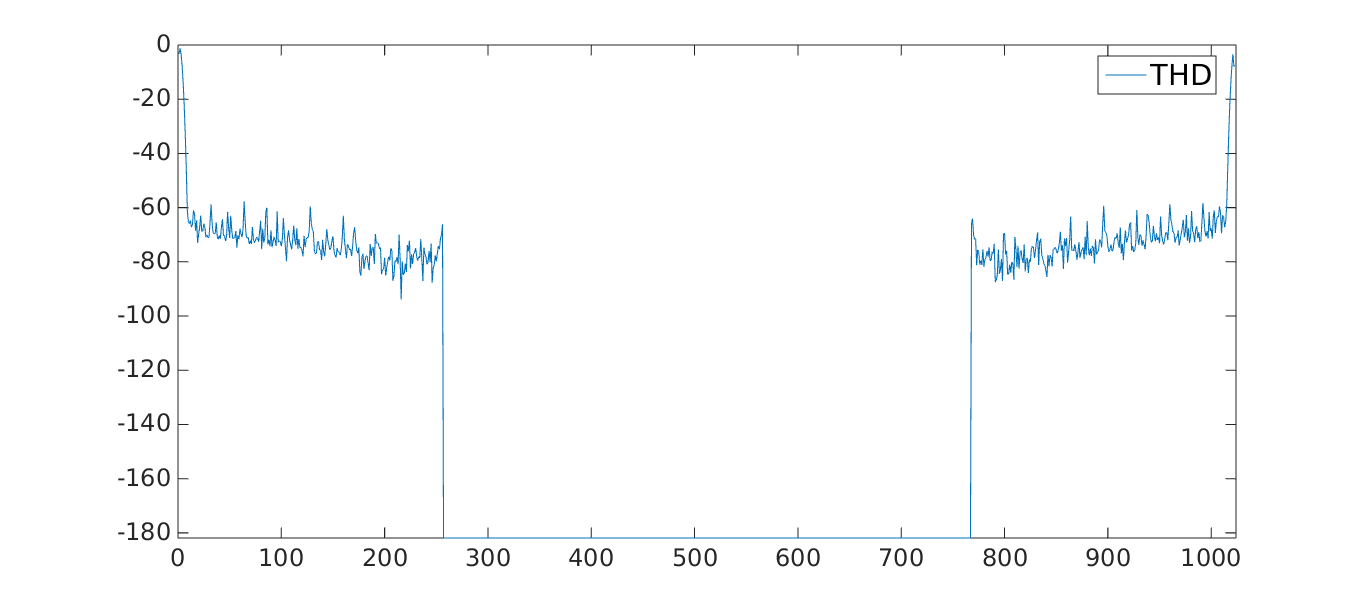
\includegraphics[width=7cm]{./figures/thd_r4_1024_12_cor.png}
        \caption{R-4, Cordic, 12 bits}
        \label{fig:r4_thd_1024_cor}
\end{figure}

\subsection{Test on Hardware}

For hardware validation, a Xilinx XC5XVL110 Virtex-5 FPGA is used. $1024$ points, $12$ bits iterative radix-2 and radix-4 are 
sinthesized with Xilinx ISE v13.4 and routed into the FPGA along with a testbench circuit wich provides PC connection via a UART port.\\
Testbench circuit is showed in Figure (\ref{fig:hw_tb}).\\

\begin{figure}[htb!]
        \centering
        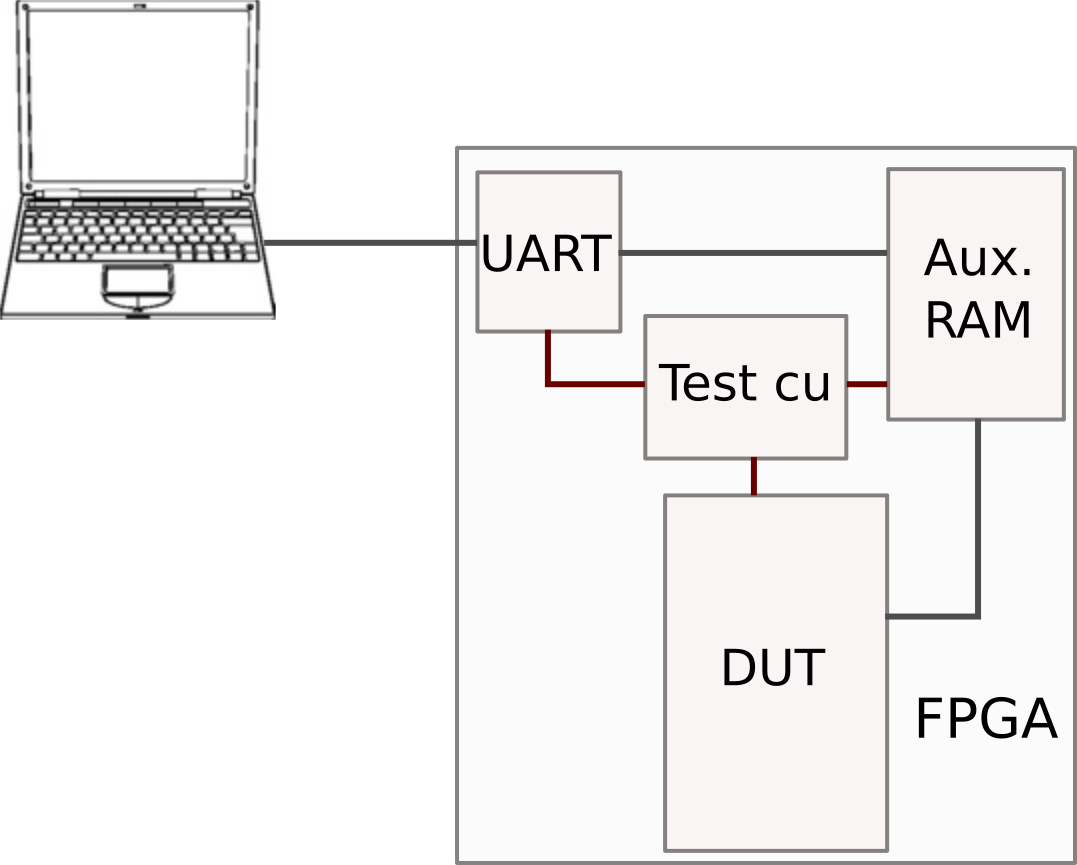
\includegraphics[width=5cm]{./figures/hw_tb.png}
        \caption{Testbench for hardware validation}
        \label{fig:hw_tb}
\end{figure}

Standard signal tests and error test, described above, are repeated on the hardware implementation obtaining the same results, 
providing the succesfull on-hardware validation of the cores.

\subsection{Resource ocupation}

The main requirement for the design is the low space/resource ocupation.\\
To validate the requirement accomplishment, $1024$ and $4096$ $16$ bits iterative radix-2 and iterativa radix-4 architectures are 
sinthesized. To have a reference for comparition, a $16$ bits radix-2 sdf (unrolled) is implemented for $1024$ and $4096$ points.
Also, as a valid testbench, Xilinx's LogiCORE FFT v7.1 \cite{fftXilinx}, is sinthesized for both point quantity.\\

\begin{figure}[htb!]
        \centering
        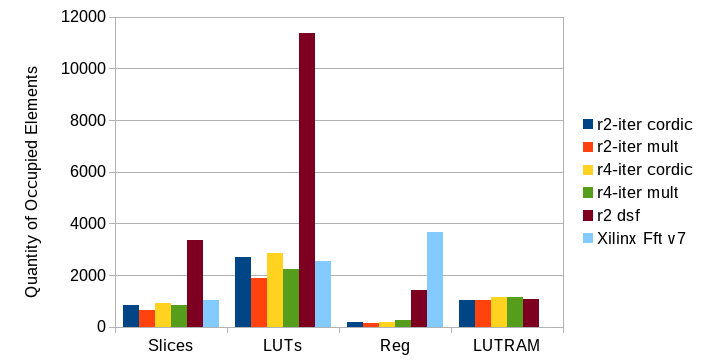
\includegraphics[width=8cm]{./figures/sizecomp1024.png}
        \caption{Size/resource comparitionComparativa for 1024 points FFT}
        \label{fig:sizecomp1024}
\end{figure}

\begin{figure}[htb!]
        \centering
        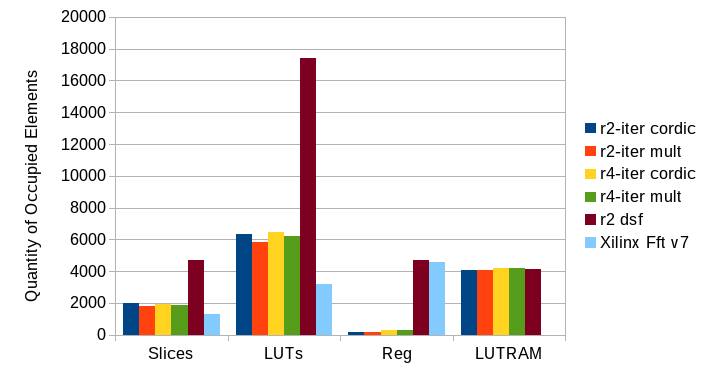
\includegraphics[width=8cm]{./figures/sizecomp4096.png}
        \caption{Size/resource comparitionComparativa for 4096 points FFT}
        \label{fig:sizecomp4096}
\end{figure}

Figures (\ref{fig:sizecomp1024}) and (\ref{fig:sizecomp4096}) clearly shows that the designed cores are really small compared 
with another implementations, inclulding a propietary, device-optimized one like the LogiCORE FFT. Another important fact is that 
radix-4 and radix-2 needs aproximated the same resources, but radix-4 has double the throughput than radix-2 (one point every 
$log_4N$ vs one point every $log_2N$).  

\section{Conclusion}
This paper presented two iterative radix-r FFT computing cores, designed for OFDM
comunication systems. Their main advantage is the extremly low space/resource comsuption, wich made the suitable for
integration in large systems without impacting in the resource distribution, in case of FPGA implementation, or space in case of
ASIC implementation. A complete description of the design and the verification and validation process has been presented.\\ 
A lot of effort was spent in the verification process, making a lot of simulations and tests, in order to provide a  
usable ip core.\\
The architectures are implemented in Verilog HDL code, comprising about 20 coding files. Also there were developed testing tools
in form of Matlab/Octave scripting, C++ programs and Verilog testbenchs.\\
For future work, can be considerated to add a dithering system, in order to reduce the noise generated by the architectures, and 
implement a pipelined cordic without modifing the global architecture timing, in order to improve the throughput. 



% trigger a \newpage just before the given reference
% number - used to balance the columns on the last page
% adjust value as needed - may need to be readjusted if
% the document is modified later
%\IEEEtriggeratref{8}
% The "triggered" command can be changed if desired:
%\IEEEtriggercmd{\enlargethispage{-5in}}

% references section

% can use a bibliography generated by BibTeX as a .bbl file
% BibTeX documentation can be easily obtained at:
% http://www.ctan.org/tex-archive/biblio/bibtex/contrib/doc/
% The IEEEtran BibTeX style support page is at:
% http://www.michaelshell.org/tex/ieeetran/bibtex/
%\bibliographystyle{IEEEtran}
% argument is your BibTeX string definitions and bibliography database(s)
%\bibliography{IEEEabrv,../bib/paper}
%
% <OR> manually copy in the resultant .bbl file
% set second argument of \begin to the number of references
% (used to reserve space for the reference number labels box)



\begin{thebibliography}{1}
\bibitem{Schaffer2_3}               Oppenheim, A., Shafer, R. (1999). The Discrete Fourier Transform. In
                                    \textit{Discrete-Time Signal Processing}, USA: Prentice Hall.
\bibitem{Prasad2_1}                 Prasad, R. (2004), Orthogonal Frequency-Division Multiplexing. 
                                    In \textit{OFDM for Wireless Communications Systems} (p.p. 11-15), UK: Artech House.
\bibitem{MeyerRadix}                Meyer-Baese, U. (2007). Fourier Transform. En \textit{Digital Signal Processing
                                    with Field Programmable Gate Arrays} (p.p. 363-373), Berlin: Springer-Verlag.
\bibitem{torkelson}                 Shousheng H., Torkelson M. (1996). A New Approach to Pipeline FFT Processor.
                                    \textit{International Parallel Processing Symposium}
\bibitem{Volder}                    Volder, J. (1959). The Cordic computer technique. \textit{IRE. Trans. Elect. Comput.}
\bibitem{BKM}                       Bajard, J.C., Kla, S., Muller, J.C. (1994, Agosto). BKM: A New Hardware Algorithm for
                                    Complex Elementary Functions. \textit{IEEE Transaction on Computers 43}(8)
\bibitem{KISSFFT}                   https://sourceforge.net/projects/kissfft/?source=navbar \textit{Kiss FFT is a very small, 
                                    reasonably efficient, mixed radix FFT library that can use either fixed or floating point data
                                    types.}
\bibitem{fftXilinx}                 LogiCORE IP Fast Fourier Transform v7.1. (2011) Xilinx
\bibitem{tesis}                     Cassagnes, A., Lutenberg, A., Giordano Zacchigna, F. (2016) ``Implementación y análisis de algoritmos
                                    de cálculo de Transformada Rápida de Fourier para su aplicación en sistemas OFDM'' 
                                    http://laboratorios.fi.uba.ar/lse/tesis/LSE-FIUBA-Tesis-Grado-Andres-Cassagnes-2016.pdf
\end{thebibliography}


\end{document}
